\ifprof
\else
%\begin{wrapfigure}{r}{7cm}
%%\begin{figure}[H]
%\centering
%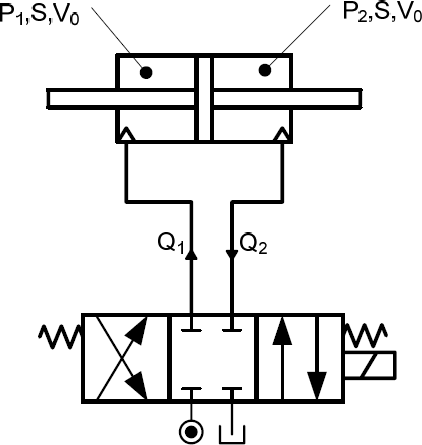
\includegraphics[width=.95\linewidth]{img_01}
%\caption{RobuROC 6 \label{fig:01}}
%%\end{figure}
%\end{wrapfigure}
Le robuROC 6 (\autoref{fig:01}) est un robot mobile développé par la société ROBOSOFT. Cette plate-forme robotisée a été conçue pour des applications de recherche et d’exploration en milieu extérieur. Elle est équipée de 6 roues motrices indépendantes, de même diamètre, montées par paires sur 3 podes articulés en tangage et en roulis (\autoref{img:03}). La cinématique permet à la plate-forme de se conformer au relief parcouru et de franchir des obstacles du type trottoirs, escaliers… Le robuROC 6 a été conçu pour se déplacer en zones urbaines et peut aussi s’adapter à tous types de milieux.  Afin d’explorer la zone géographique à risques, les 3 podes peuvent être équipés, selon les besoins de l’utilisateur, de caméras d’observation haute définition à 360\degres, de systèmes infrarouges de visualisation nocturne, ainsi que de bras de robot articulés pour manipuler des éléments de la zone à explorer. Les diagrammes de contexte %SADT A-0 
(\autoref{fig:011}) et %FAST 
le diagramme des exigences (annexe 1) recensent les fonctions remplies par la plate-forme.


\begin{minipage}[c]{.47\linewidth}
\begin{figure}[H]
\centering
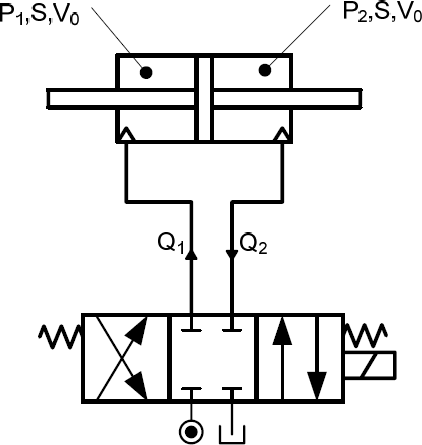
\includegraphics[width=.8\linewidth]{img_01}
\caption{RobuROC 6 \label{fig:01}}
\end{figure}
\end{minipage} \hfill
\begin{minipage}[c]{.47\linewidth}
\begin{figure}[H]
\centering
%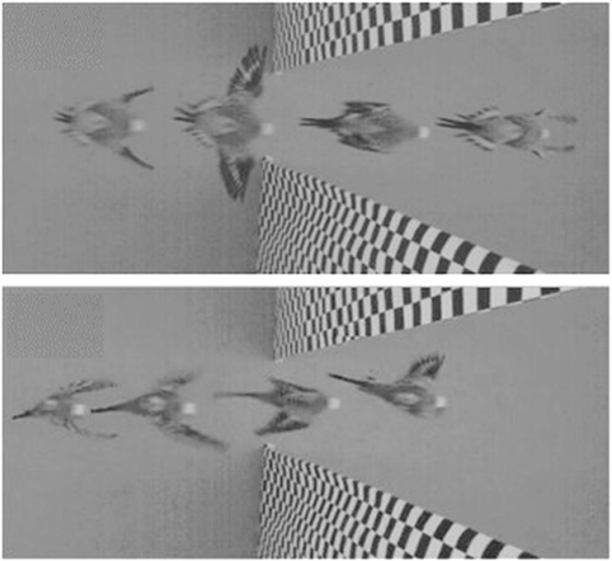
\includegraphics[width=.95\linewidth]{fig_01}
%\caption{SADT A-0  \label{fig:011}}
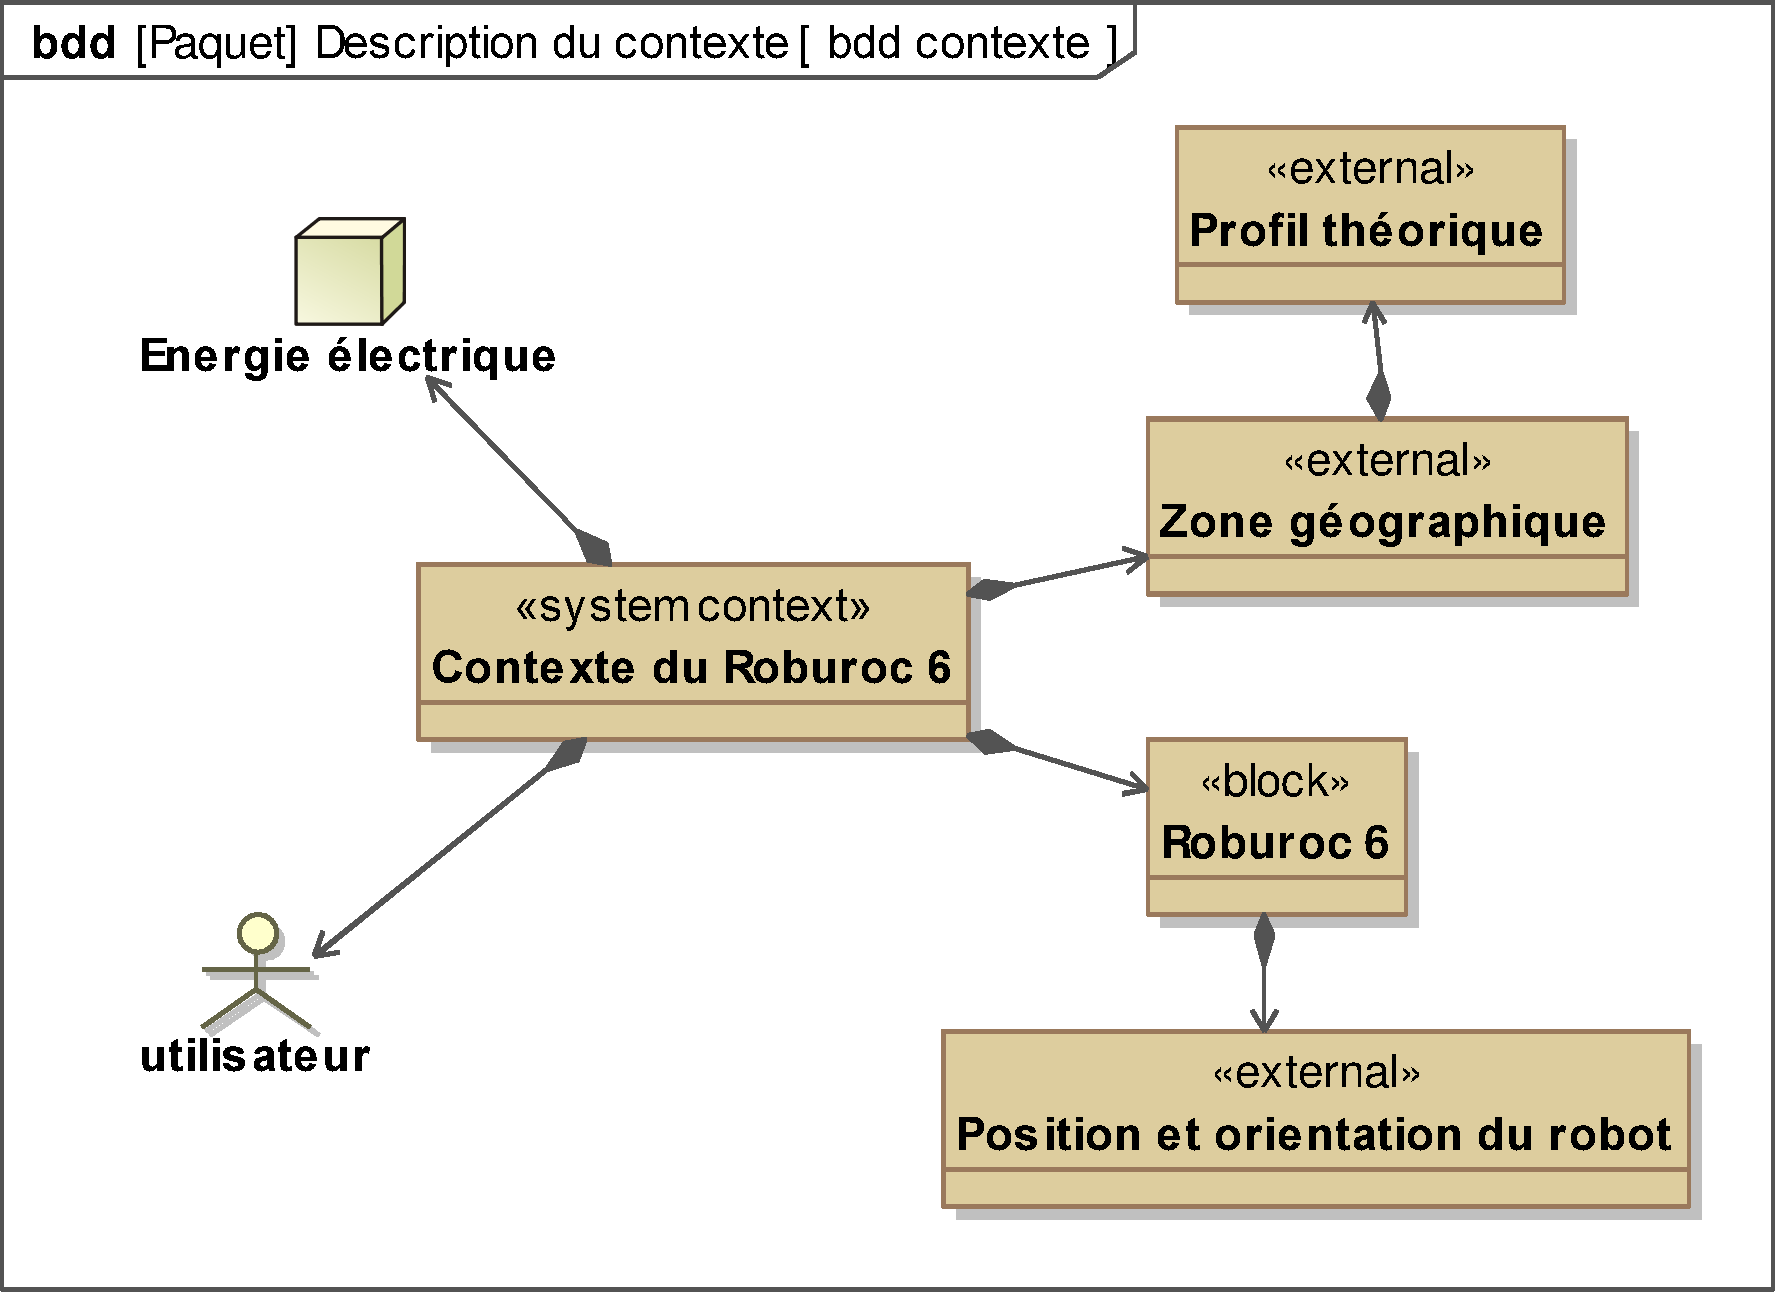
\includegraphics[width=.95\linewidth]{img_bdd}
\caption{Diagramme de contexte  \label{fig:011}}

\end{figure}
\end{minipage} 

\vspace{.5cm}

Les déplacements de la plate-forme sont coordonnés par l’intermédiaire de deux microcontrôleurs placés dans les podes avant et arrière. Ces microcontrôleurs communiquent entre eux et dialoguent avec l’extérieur suivant deux modes de conduite : 
\begin{itemize}
\item le mode joystick : l’utilisateur pilote manuellement la plate-forme par l’intermédiaire d’une télécommande;
\item le mode automatique : la plate-forme traite les informations du logiciel de supervision notamment le suivi d’un profil théorique.
\end{itemize}

Pour se repérer dans l’espace, la plate-forme est équipée de capteurs relatifs positionnés sur chacune des six roues, d’inclinomètres et d’un système de positionnement absolu par GPS. Des capteurs à ultrasons et des « bumpers » (détecteurs de collision) participent à la sécurité matérielle et à la détection des obstacles.
La motorisation principale est assurée par six moteurs électriques équipés de réducteurs épicycloïdaux permettant de transmettre l’énergie mécanique aux six roues. Le franchissement des obstacles est facilité par un système hydraulique permettant le soulèvement des podes avant et arrière. Ce système est constitué de quatre vérins disposés de part et d’autre du pode central (\autoref{img:03}) et d’une centrale hydraulique alimentée par une pompe à engrenage (annexe 2). La plate-forme peut se déplacer, sous conditions, en mode 6 roues ou 4 roues pour certaines applications particulières (\autoref{fig:02}). L’énergie électrique nécessaire au fonctionnement est stockée dans des batteries occupant la plus grande partie du volume interne des trois podes. Une unité de gestion électrique optimise la consommation d’énergie. 

\begin{figure}[H]
\centering
\begin{subfigure}{0.27\textwidth}
    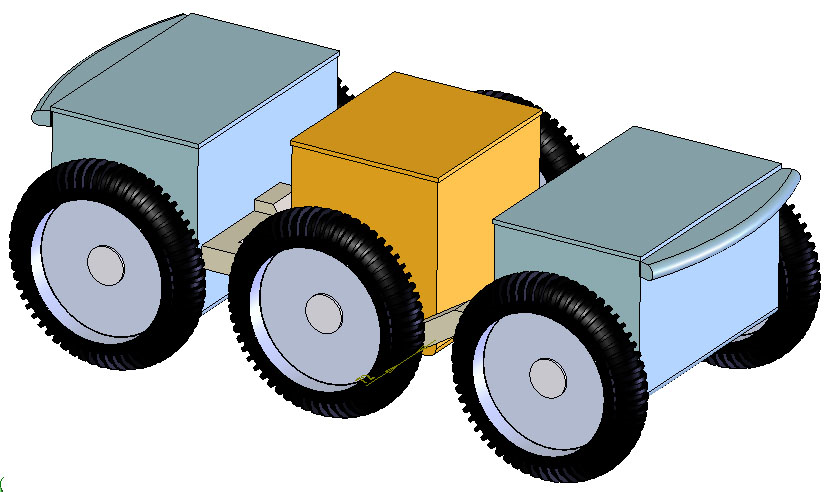
\includegraphics[width=\linewidth]{img_02_a}
    \caption{Mode 6 roues}
    \label{fig:02a}
\end{subfigure} \hfill
\begin{subfigure}{0.27\textwidth}
    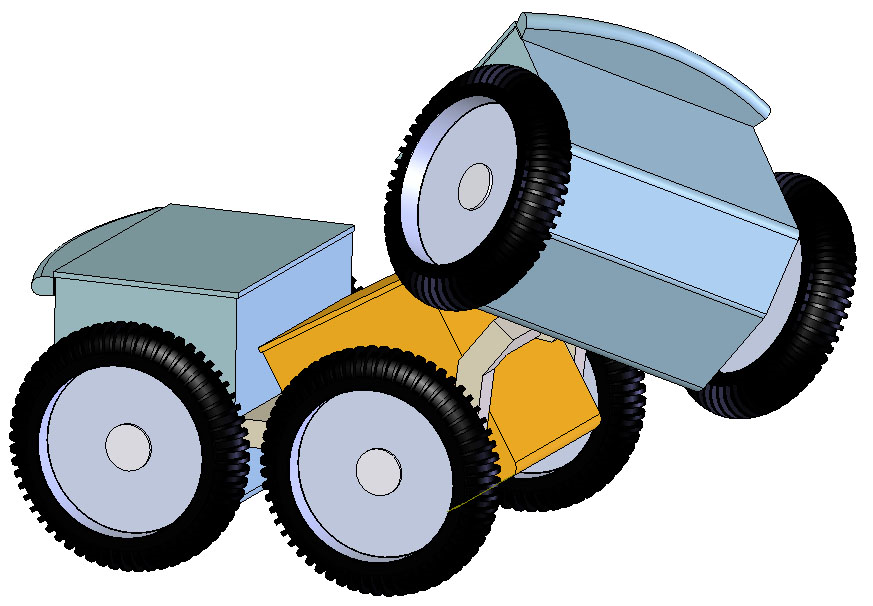
\includegraphics[width=\linewidth]{img_02_b}
    \caption{Mode 4 roues -- Déplacement}
    \label{fig:02a}
\end{subfigure} \hfill
\begin{subfigure}{0.27\textwidth}
    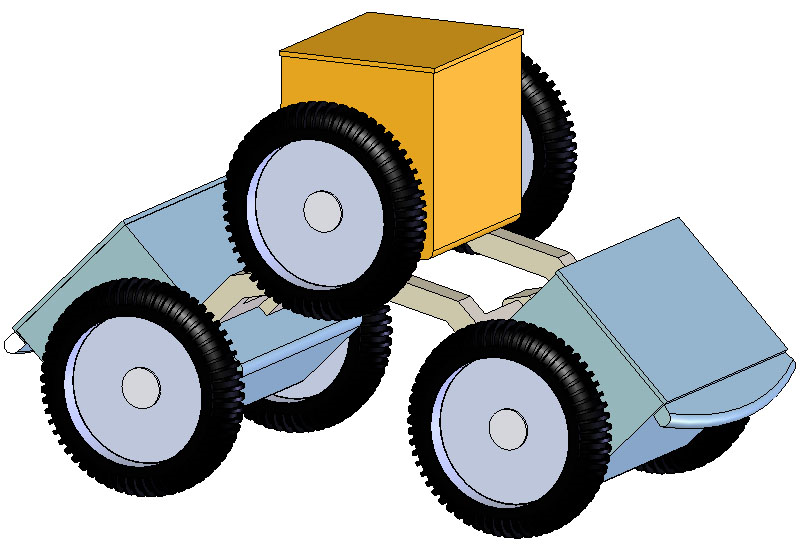
\includegraphics[width=\linewidth]{img_02_c}
    \caption{Mode 4 roues -- Observation}
    \label{fig:02a}
\end{subfigure}\caption{Mode de déplacement de la plate-forme \label{fig:02}}
\end{figure}


\begin{figure}[H]
\centering
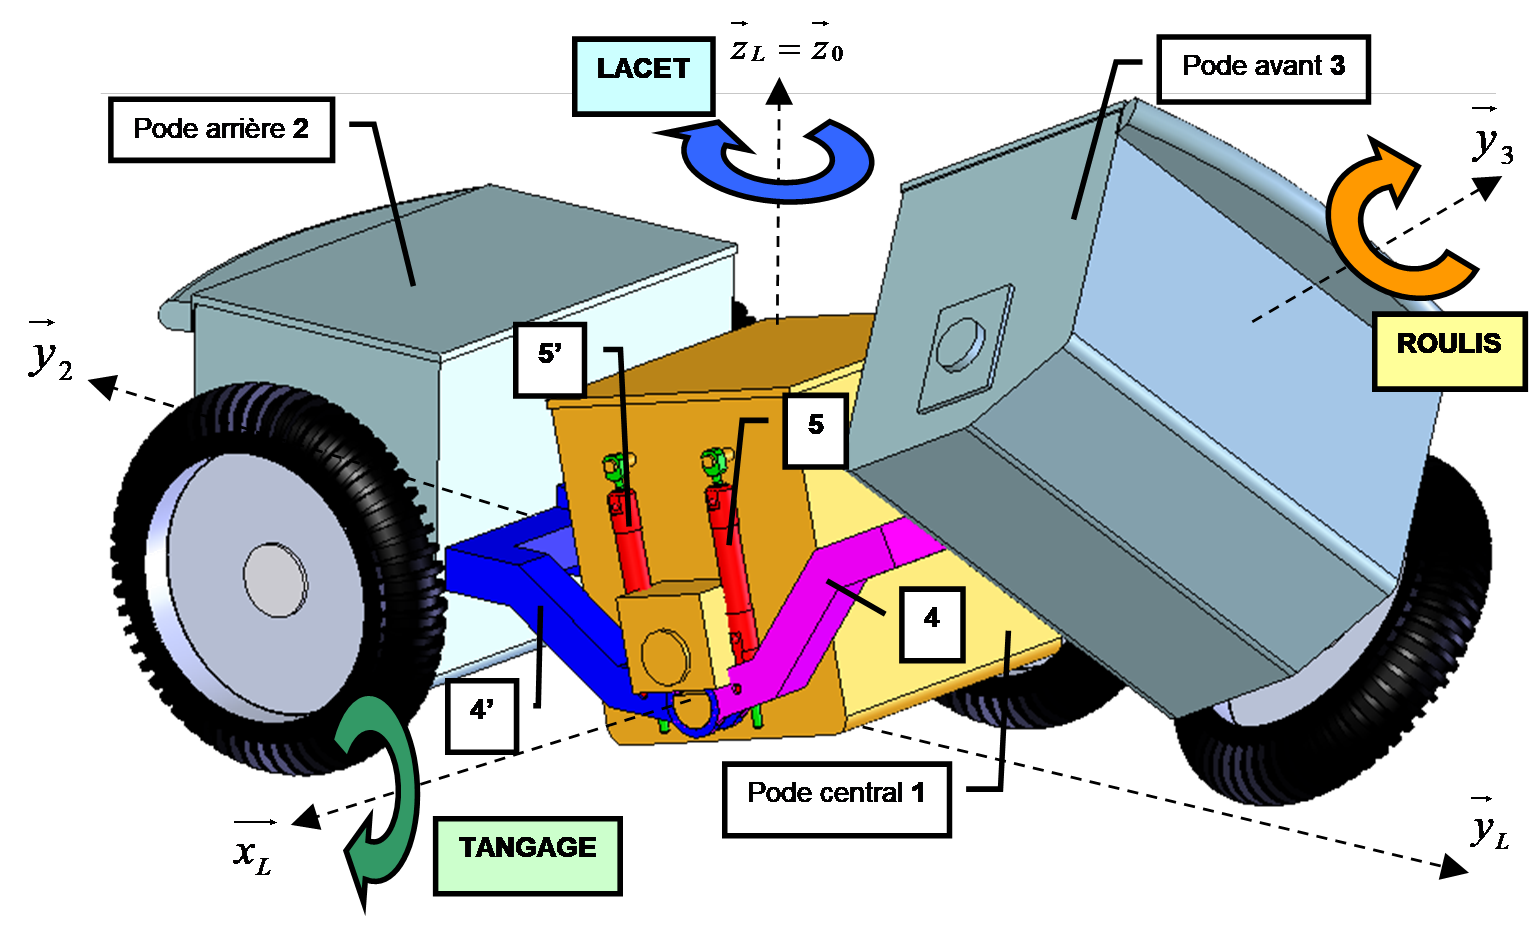
\includegraphics[width=.6\linewidth]{img_03}
\caption{Roue centrale et roue avant droite supprimées pour plus de visibilité \label{img:03}}
\end{figure}

Les trois podes sont articulés en tangage et en roulis (\autoref{img:03}). Le mouvement de tangage est guidé par deux liaisons pivot (d’axe de direction  $\vect{x_L}$), respectivement entre le bras d’articulation avant \textbf{4} et le pode central \textbf{1} et entre le bras d’articulation arrière \textbf{4’} et le pode central \textbf{1}. Le système hydraulique de suspension permet l’amortissement (mode passif) et la motorisation de ce mouvement (mode actif). Les vérins \textbf{5} (côté droit) et \textbf{6} (côté gauche) sont en liaison avec le bras d’articulation avant \textbf{4} et le pode central \textbf{1}. Les vérins \textbf{5’} (côté droit) et \textbf{6’} (côté gauche) sont en liaison avec le bras d’articulation arrière \textbf{4’} et le pode central \textbf{1}. Le mouvement de roulis est assuré par deux liaisons pivot entre le pode avant \textbf{3} et le bras d’articulation avant \textbf{4} (liaison d’axe de direction $\vect{y_3}$) d’une part, et entre le pode arrière \textbf{2} et le bras d’articulation arrière \textbf{4’}  (liaison d’axe de direction $\vect{y_2}$) d’autre part. Ce mouvement n’est pas motorisé. 

%\begin{table}[H]
%\centering
%\begin{tabular}{|p{4cm}|p{6cm}|l|l|}
%\hline
%Fonctions & Critères & Niveaux & Flexibilité \\ 
%\hline
%\hline
%\multirow{7}{4cm}{FT3 : Assurer le déplacement}
% & Vitesse de déplacement de la plate-forme & $\SI{13,7}{km/h}$ & Valeur maximale \\ \cline{2-4}
% & Hauteur de franchissement d’un obstacle de type « trottoir » ($D_{\text{max}}$) & \SI{40}{cm} & Valeur minimale  \\ \cline{2-4}
% & Pente du relief à vide & 45\degres & Valeur maximale  \\ \cline{2-4}
% & Débattement angulaire en tangage du bras 4 par rapport au pode central 1 & de $-45\degres$ à $+30\degres$ & -----  \\ \cline{2-4}
% & Débattement angulaire en tangage du bras 4’ par rapport au pode central 1 & de $+45\degres$ à $-30\degres$ & ----- \\ \cline{2-4}
% & Débattement angulaire en roulis du pode avant 3 par rapport au bras 4 & de $-45\degres$ à $+45\degres$ & ----- \\ \cline{2-4}
% & Débattement angulaire en roulis du pode arrière 2 par rapport au bras 4’ & de $+45\degres$ à $-45\degres$ & ----- \\
% \hline
% \multirow{2}{4cm}{FT4 : Analyser la zone géographique à explorer}
% & Charge utile répartie sur les trois podes & \SI{100}{kg} & Valeur maximale \\ \cline{2-4}
% & Hauteur d’observation ($H_{\text{obs}}$) & \SI{85}{cm} & Valeur minimale \\ \hline
%FT6 : Fournir l’énergie électrique & Autonomie d’utilisation $\SI{4}{h} $ & $\pm \SI{1}{h}$ &Selon les conditions \\ \hline
%\end{tabular}
%\caption{Extrait du cahier des charges fonctionnel (d’après le diagramme FAST en annexe 1)}
%\end{table}

\begin{table}[H]
\centering
\begin{tabular}{p{4cm}p{6cm}ll}
\hline
Exigences fonctionnelles & Critères & Niveaux & Flexibilité \\ 
\hline
%\hline
\multirow{7}{4cm}{Id 1.3 : Assurer le déplacement}
 & Vitesse de déplacement de la plate-forme & $\SI{13,7}{km/h}$ & Valeur maximale \\ %\cline{2-4}
 & Hauteur de franchissement d’un obstacle de type « trottoir » ($D_{\text{max}}$) & \SI{40}{cm} & Valeur minimale  \\ %\cline{2-4}
 & Pente du relief à vide & 45\degres & Valeur maximale  \\ %\cline{2-4}
 & Débattement angulaire en tangage du bras 4 par rapport au pode central 1 & de $-45\degres$ à $+30\degres$ & -----  \\ %\cline{2-4}
 & Débattement angulaire en tangage du bras 4’ par rapport au pode central 1 & de $+45\degres$ à $-30\degres$ & ----- \\ %\cline{2-4}
 & Débattement angulaire en roulis du pode avant 3 par rapport au bras 4 & de $-45\degres$ à $+45\degres$ & ----- \\ %\cline{2-4}
 & Débattement angulaire en roulis du pode arrière 2 par rapport au bras 4’ & de $+45\degres$ à $-45\degres$ & ----- \\ \hline
 \multirow{2}{4cm}{Id 1.4 : Analyser la zone géographique à explorer}
 & Charge utile répartie sur les trois podes & \SI{100}{kg} & Valeur maximale \\ %\cline{2-4}
 & Hauteur d’observation ($H_{\text{obs}}$) & \SI{85}{cm} & Valeur minimale \\ \hline
Id 1.6 : Fournir l’énergie électrique & Autonomie d’utilisation $\SI{4}{h} $ & $\pm \SI{1}{h}$ &Selon les conditions \\ \hline
\end{tabular}
\caption{Extrait du cahier des charges fonctionnel (d’après le diagramme des exigences en annexe 1)}
\end{table}

\fi

%\section{Analyse fonctionnelle \label{sec:1}}
\section{Analyse des exigences \label{sec:1}}
%\question{\label{q_01} Compléter le diagramme FAST de la plate-forme d’exploration présenté en annexe 1 en indiquant les solutions techniques associées aux fonctions techniques référencées dans le tableau du document-réponse. Pour cela, vous associerez aux fonctiosn techniques FT1, FT2, FT311, FT312, FT321, FT33, FT41, FT51, FT61, FT71.}
\question{\label{q_01} Compléter le diagramme des exigencs de la plate-forme d’exploration présenté en annexe 1 en indiquant les solutions techniques associées aux fonctions techniques référencées dans le  document-réponse.}% Pour cela, vous associerez aux fonctiosn techniques FT1, FT2, FT311, FT312, FT321, FT33, FT41, FT51, FT61, FT71.}
\ifprof
\begin{corrige}
\end{corrige}
\else
\fi



%\section{Fonction technique FT32 : Assurer le mouvement en tangage \label{sec:2}}
\section{Exigence fonctionnelle ID 1.3.2 : Assurer le mouvement en tangage \label{sec:2}}

\begin{hypo}~\\
\begin{itemize}
\item Dans toute la partie II, le mouvement de roulis est fixé à une valeur nulle. Ainsi le bras d’articulation avant \textbf{4} et le pode avant \textbf{3} sont solidaires et de la même manière, le bras d’articulation arrière \textbf{4’} et le pode arrière \textbf{2} sont aussi solidaires. D’autre part, le mouvement de lacet n’est pas considéré.
\item Les éléments hydrauliques placés du côté gauche (vérins \textbf{6} et \textbf{6’}) agissent exactement de la même manière que les éléments placés du côté droit (vérins \textbf{5} et \textbf{5’}). L’étude suivante du circuit hydraulique sera donc réalisée uniquement du côté droit.
\end{itemize}
\end{hypo}

\subsection{Fonctionnement du circuit hydraulique}
\ifprof
\else
Les fonctions à remplir par le circuit hydraulique (annexe 2) sont principalement de :
\begin{itemize}
\item synchroniser les mouvements de tangage des podes avant et arrière afin de se conformer au relief ;
\item amortir les mouvements de tangage ;
\item piloter les mouvements de tangage.
\end{itemize}
\fi

\subsubsection{Synchroniser et amortir les mouvements de tangage des trois podes}
\ifprof
\else

Dans un premier temps, la centrale hydraulique n’est pas activée (annexe 2). Il s’agit donc d’étudier le comportement
de la plate-forme en mode passif (suivi du relief et amortissement des mouvements sans pilotage).
Les vérins utilisés, tous identiques, sont des vérins à double effet et tige traversante. Chaque vérin possède deux
chambres à volume variable remplies d’huile. Deux répartiteurs hydrauliques (un répartiteur placé du côté gauche et
l’autre du côté droit) assurent la circulation de l’huile entre les vérins avant et arrière en croisant l’alimentation des
chambres des vérins avant et arrière.

Un schéma cinématique du montage des vérins est fourni en annexe 3 et est complété par la représentation des
principales fonctionnalités du répartiteur hydraulique droit.
\fi


\question{\label{q_02}Sur le document-réponse (questions \ref{q_02} et \ref{q_03}), indiquer en hachurant, les chambres des vérins qui sont en communication ainsi que le flexible permettant de les relier. Vous adopterez un type de hachures par volume d’huile en communication.}
\ifprof
\begin{corrige}
\end{corrige}
\else
\fi

\ifprof
\else

À partir d’une position plane de la plate-forme (position du document-réponse questions \ref{q_02} et \ref{q_03}), considérons que le pode avant \textbf{3} commence un mouvement de CABRAGE (montée du pode avant \textbf{3} et du bras d’articulation \textbf{4} par rapport au pode central \textbf{1}) suite à un obstacle. On note $\beta$ l’angle de tangage entre le bras d’articulation \textbf{4} et le pode central \textbf{1} engendré par ce mouvement.
\fi

\question{\label{q_03}Sur le document-réponse (questions \ref{q_02} et \ref{q_03}), indiquer par des flèches le sens de circulation de l’huile dans les flexibles au cours de ce mouvement de CABRAGE. Indiquer quel est le mouvement engendré entre l’ensemble \{pode arrière \textbf{2} + bras d’articulation \textbf{4’}\} et le pode central \textbf{1}, ainsi que son amplitude suite au mouvement de CABRAGE du pode avant d’un angle $\beta$.}
\ifprof
\begin{corrige}
\end{corrige}
\else
\fi


\subsubsection{Piloter les mouvements de tangage}
\ifprof
\else

Le système hydraulique est conçu de telle sorte que les angles de tangage entre le pode central \textbf{1} d’une part et les
podes avant / arrière d’autre part soient opposés à chaque instant. Ainsi, l’utilisateur n’a besoin de définir qu’un seul
angle de tangage $\beta$ défini entre le pode central \textbf{1} et le pode avant \textbf{3} par $\beta=\angl{y_1}{y_3}=\angl{z_1}{z_3}$ (annexe 5). L’angle
$\beta$
varie entre $- 45\degres$ et $+30\degres$. Les valeurs négatives correspondent à un mouvement de PLONGEE du pode avant, les
valeurs positives à un mouvement de CABRAGE.

Afin de piloter l’angle de tangage $\beta$ conformément aux consignes des microcontrôleurs, la centrale hydraulique est activée. Un schéma de principe de cette centrale est fourni sur le document-réponse (question \ref{q_04}). La circulation d’huile est générée par une pompe à engrenage entraînée par un moteur électrique. Les consignes électriques de CABRAGE ou de PLONGEE agissent sur un distributeur 4/3 (4 orifices et 3 positions) afin de réaliser le mouvement attendu au niveau des vérins (description du fonctionnement et de la normalisation d’un distributeur 4/3 disponible en annexe 4).
\fi

\question{\label{q_04} Sur le document-réponse (question \ref{q_04}), relier les orifices de sortie du distributeur 4/3 aux flexibles
d’alimentation des vérins afin de respecter les ordres de PLONGEE et de CABRAGE.}
\ifprof
\begin{corrige}
\end{corrige}
\else
\fi



\subsection{Validation des performances du circuit hydraulique}
\ifprof
\else

La position de PLONGEE maximale, permet au pode central \textbf{1} d’atteindre son point culminant par rapport au sol. Seuls les podes avant \textbf{3} / arrière \textbf{2} sont alors en contact avec le sol horizontal. Cette position, appelée « Mode 4 roues Observation » (\autoref{fig:02}), permet à l’utilisateur d’observer le milieu environnant à l’aide d’une caméra placée sur le plan supérieur du pode central. La position de CABRAGE maximale, permet quant à elle de soulever le pode avant le plus haut possible afin de franchir un obstacle (« Mode 4 roues Déplacement » (\autoref{fig:02})). Dans cette position, seuls le pode arrière \textbf{2} et le pode central \textbf{2} sont en contact avec le sol.
\fi

\subsubsection{Etude du CABRAGE}
\ifprof
\else


Sur le document-réponse (question \ref{q_05}), le pode central \textbf{1} est représenté en « Mode 4 roues Déplacement ». Les podes \textbf{2} et \textbf{3} ont été représentés en pointillés dans leur position initiale pour un angle de tangage nul. Les points $C_{3i}$ et $C_{2i}$ définissent respectivement les positions initiales du centre de la roue avant et du centre de la roue arrière.
\fi

\question{\label{q_05}Représenter, sur le document-réponse (question \ref{q_05}), pour la position de CABRAGE maximal ($\beta_{\text{max}}=30\degres$) :
\begin{itemize}
\item les positions du centre de la roue avant, appelé $C_{3C}$ et du centre de la roue arrière, appelé $C_{2C}$;
\item les cercles représentant les roues avant et arrière ainsi qu’une droite représentant le sol ;
\item la hauteur de franchissement maximal $D_{\text{max}}$ mesurée perpendiculairement au sol jusqu’au bas de la roue avant.
\end{itemize}
Mesurer $D_{\text{max}}$ et comparer cette valeur au cahier des charges.}
\ifprof
\begin{corrige}
\end{corrige}
\else
\fi


\subsubsection{Dimensionnement des vérins}
\ifprof
\else

Le choix des vérins assurant le mouvement de tangage est délicat. En effet, l’encombrement très réduit oblige le
concepteur à positionner l’axe de fixation des vérins avec les bras \textbf{4} et \textbf{4’} très près de l’axe de rotation en tangage $\axe{O_1}{x_L}$. L’objectif de cette partie est de déterminer la course des vérins en fonction de l’amplitude du mouvement ainsi que la pression maximale $p_{\text{maxi}}$ dans le circuit hydraulique. Pour cette étude, nous considèrerons la configuration d’essai suivante où le pode central \textbf{1} est fixe et placé parallèlement au sol. L’ensemble E=\{bras d’articulation avant \textbf{4} + pode avant \textbf{3} + roues avant\} est soulevé par les vérins avant \textbf{5} et \textbf{6} placés de part et d’autre du pode central \textbf{1}. Le modèle cinématique retenu est défini sur \textbf{l’annexe 6}.

Le mécanisme est constitué : 
\begin{itemize}
 \item du pode central fixe \textbf{1} : repère associé $\rep{1}=\repere{O_1}{x_1}{y_1}{z_1}$;
 \item de l'ensemble  E=\{bras d’articulation avant \textbf{4} + pode avant \textbf{3} + roues avant\} : repère associé $\rep{3}=\repere{O_1}{x_1}{y_3}{z_3}$ avec $\beta = \axe{y_1}{y_3} =\axe{z_1}{z_3}$;
 \item du vérin \textbf{4} constitué du corps \textbf{$5_1$} et de la tige \textbf{$5_2$} : repère associé $\rep{5}=\repere{A}{x_1}{y_5}{z_5}$ avec
  $\gamma = \axe{y_3}{y_5}= \axe{z_3}{z_5}$;
 \item du vérin \textbf{6} non représenté car ayant le même comportement que le vérin \textbf{5}.
\end{itemize}

\textbf{Paramétrage :}
\begin{itemize}
 \item $\vect{O_1 A}=d_4\vect{y_3}$, $\vect{AB}=\lambda\vect{y_5}$, $\vect{O_1 B}=d_1\vect{y_1}+h_1\vect{z_1}$.
\end{itemize}

Valeurs numériques : 
\begin{itemize}
 \item $d_4 =\SI{70}{mm}$; $h_1 =\SI{292}{mm}$; $d_1 =\SI{76}{mm}$; $\beta \in \left[ -45\degres;+30\degres\right]$.
\end{itemize}
\fi

\question{Exprimer $\lambda$ en fonction de $d_4$, $h_1$, $d_1$ et $\beta$.}
\ifprof
\begin{corrige}
\begin{itemize}
\item On commence par écrire la fermeture géométrique : $\vect{O_1A}+\vect{AB}+\vect{BO_1} = \vect{0}$ 
$ \Leftrightarrow d_4\vect{y_3} +\lambda\vect{y_5} - d_1\vect{y_1}-h_1\vect{z_1} = \vect{0}$.
\item On projette la relation vectorielle dans le repère $\rep{1}$ :
$\left\{
\begin{array}{l}
d_4\cos\beta +\lambda\cos(\beta+\gamma) - d_1= {0}  \\
d_4\sin\beta +\lambda\sin(\beta+\gamma) - h_1= {0}  \\
\end{array}
\right.$
\item On cherche à éliminer $\gamma$ :
$\left\{
\begin{array}{l}
\lambda\cos(\beta+\gamma) =d_1 - d_4\cos\beta  \\
\lambda\sin(\beta+\gamma)  = h_1  - d_4\sin\beta \\
\end{array}
\right.$ 
$ \Rightarrow \left\{
\begin{array}{l}
\lambda^2\cos^2(\beta+\gamma) =\left(d_1 - d_4\cos\beta \right)^2 \\
\lambda^2\sin^2(\beta+\gamma)  =\left( h_1  - d_4\sin\beta\right)^2 \\
\end{array}
\right.$ 
\item Au final \fbox{$\Rightarrow \lambda^2  =\left(d_1 - d_4\cos\beta \right)^2 + \left( h_1  - d_4\sin\beta\right)^2$}.
\end{itemize}
\end{corrige}
\else
\fi



\question{Calculer les valeurs numériques d’élongation minimale $\lambda_{\text{min}}$, maximale $\lambda_{\text{max}}$ ainsi que la course du vérin \textbf{5}.}
\ifprof
\begin{corrige}
\begin{figure}[H]
\centering
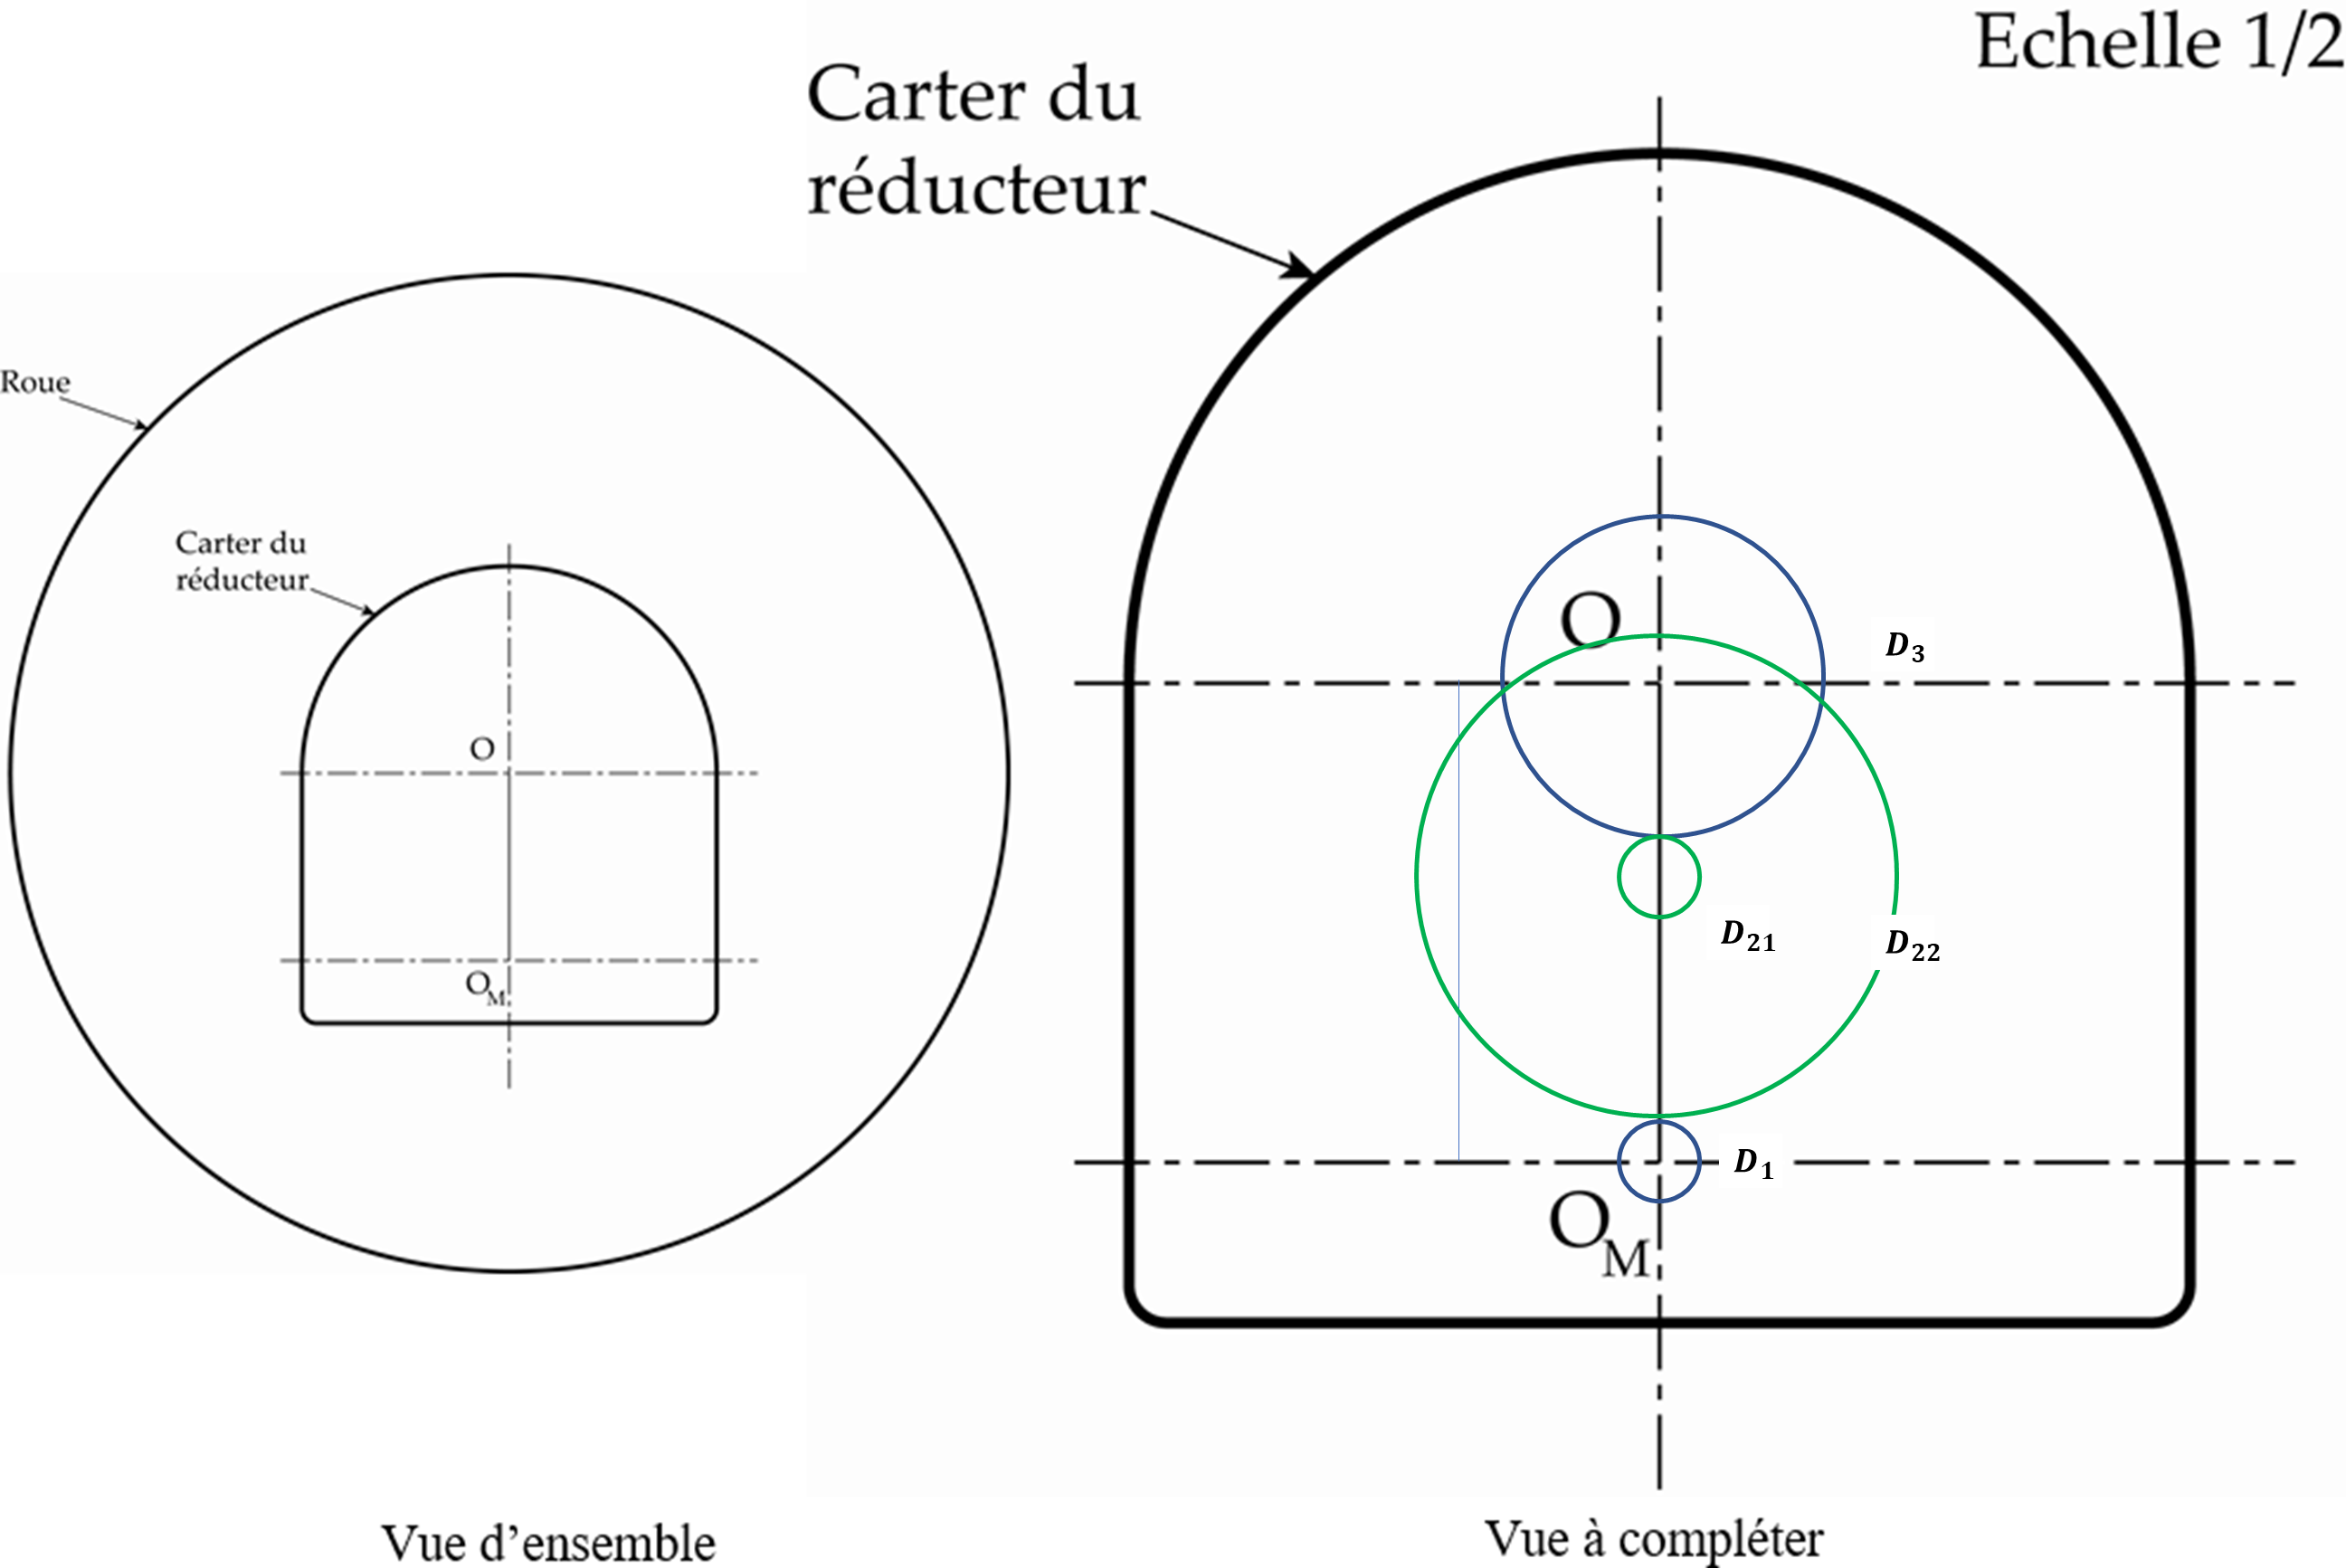
\includegraphics[width=.6\linewidth]{cor_07.png}
%\caption{Loi de commande de vitesse \label{img:04}}
\end{figure}
On observe que le maximum de la course est pour $\beta=-45\degres$ et le minimum $\beta=30\degres$.

On a $\text{Course} = \lambda_{\text{max}}-\lambda_{\text{min}} = 342,5 - 257,5 = \SI{85}{mm}$.
\end{corrige}
\else
\fi



L’objectif suivant est d’évaluer les pressions maximales s’exerçant dans le circuit hydraulique dans la configuration
d’essai décrite précédemment à savoir :
\begin{itemize}
\item le pode central \textbf{1} est fixe et placé parallèlement au sol ;
\item les podes avant \textbf{3} et arrière \textbf{2} ne sont pas en contact avec le sol et un angle de tangage est alors imposé aux podes avant et arrière par rapport au pode central.
\end{itemize}
Sur l’annexe 8, l’évolution du rapport entre les efforts exercés par les vérins avant \textbf{5} et \textbf{6} et le poids de l’ensemble E a été tracée en fonction de l’angle de tangage $\beta$. La masse de l’ensemble E est $m_E = \SI{60}{kg}$.

\question{À partir du tracé de l’annexe 8 et du plan du vérin annexe 7, déterminer la valeur de la différence de
pression maximale $\Delta P_{\text{max}}$ entre les deux chambres des vérins avant \textbf{5} et \textbf{6}.}
\ifprof
\begin{corrige}~\\
\begin{figure}[H]
\centering
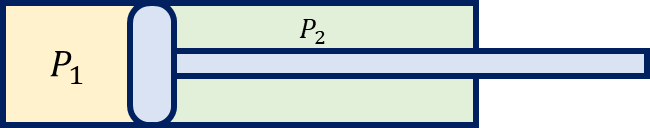
\includegraphics[width=.5\linewidth]{cor_09.png}
%\caption{Loi de commande de vitesse \label{img:04}}
\end{figure}
 
 On a $F_{\text{max}}=\Delta P_{\text{max}}\dfrac{\pi\left( D^2-d^2\right)}{4}$ et 
 $\Delta P_{\text{max}} = F_{\text{max}} \dfrac{4}{\pi\left( D^2-d^2\right)}$.
 D'aprés l'annexe, lorsque $\beta = -45\degres$, $\dfrac{F_{v5}+F_{v6}}{m_E g}=8,4$.
 
 En faisant l'hypothèse que la masse à lever se répartit équitablement sur les deux vérins, 
 $\dfrac{2F_{\text{max}}}{m_E g}=8,4$ et donc 
 $\Delta P_{\text{max}} = 8,4\cdot m_E g \dfrac{4}{2\pi\left( D^2-d^2\right)}=  \dfrac{16,8 m_E g}{\pi\left( D^2-d^2\right)}$.
 
 
 \textit{Application numérique }
  $\Delta P_{\text{max}} = \SI{60}{MPa} = \SI{600}{bar}$.
%On a dans la chambre de gauche, $p_1 = \dfrac{F_1}{S_1}$. Dans la chambre de droite, $p_2 = \dfrac{F_2}{S_2}$. On a donc $\Delta P_{\text{max}} = |p_1 - p_2| = \left| \dfrac{F_1}{S_1} - \dfrac{F_2}{S_2} \right|$
% $= \left| \dfrac{F_1}{\dfrac{\pi D^2}{4}} - \dfrac{F_2}{\dfrac{\pi\left( D^2-d^2\right)}{4}} \right|$
% $= \dfrac{4}{\pi}\left| \dfrac{F_1}{ D^2} - \dfrac{F_2}{\left( D^2-d^2\right)} \right|$
% $= \dfrac{4}{\pi}\left| \dfrac{F_1}{ D^2} - \dfrac{F_2}{D^2-d^2} \right|$
%  $= 4\dfrac{\left| F_1\left( D^2-d^2\right) - F_2D^2\right|}{\pi\left( D^2-d^2\right)D^2}$
%$ = p_1 \dfrac{\pi D^2}{4}$.
%
%$= p_2 \dfrac{\pi\left( D^2-d^2\right)}{4}$.


\end{corrige}


\else
\fi



La pression minimale dans le circuit hydraulique est supposée constante et égale à $p_0$ ( $p_0 = \SI{1}{bar}$). Des limiteurs de pression tarés à \SI{150}{bars} sont placés en sortie du distributeur 4/3.

\question{Déterminer l’expression de la pression maximale $p_{\text{maxi}}$ dans le circuit hydraulique en fonction de $p_0$ et $\Delta P_{\text{max}}$. Réaliser l’application numérique et comparer cette valeur à la pression de tarage des limiteurs.}
\ifprof
\begin{corrige}
D'après les questions précédentes, les deux vérins sont en série. On a donc $p_{\text{maxi}} - p_0 = 2 \Delta P_{\text{max}}$ soit 
$p_{\text{maxi}} = 2 \Delta P_{\text{max}} + p_0 = \SI{1201}{bar}$... chercher l'erreur.
\end{corrige}
\else
\fi


%\section{\label{sec:3}Fonction technique FT31 : Assurer le mouvement de lacet}
\section{\label{sec:3}Exigence technique 1.3.1 : Assurer le mouvement de lacet}

\begin{hypo}%Hypothèses :

\begin{itemize}
\item De la même manière que dans la partie \ref{sec:2}, dans toute la partie \ref{sec:3}, le mouvement de roulis n’est pas considéré. Il est fixé à une valeur nulle.
\end{itemize}
\end{hypo}

\ifprof
\else

Les 6 roues de la plate-forme (notée $\text{PF}$) sont motorisées permettant ainsi de se déplacer sur des reliefs très
accidentés. Cependant, la plate-forme ne comporte pas de systèmes spécifiques de direction. Le changement de
direction est imposé par une rotation différentielle des roues du pode central \textbf{1}. Les roues avant et arrière doivent alors avoir des vitesses de rotation compatibles avec celles du pode central \textbf{1}. Lorsque le rayon de courbure de la trajectoire suivie par la plate-forme devient inférieur à 4 mètres, le groupe hydraulique est actionné pour passer en « Mode 2 roues instable ». La plate-forme ne tenant pas en équilibre sur 2 roues, elle retombe dès le début du mouvement sur les roues arrière ou les roues avant, passant donc en « Mode 4 roues Déplacement ». Cette intervention du groupe hydraulique permet ainsi de soulager le contact entre les roues des podes avant / arrière et le sol. Pour cette étude, nous considèrerons que la plate-forme retombe sur les roues arrière (annexe 9) et nous nous placerons dans le cas d’un rayon de courbure nul. Le mouvement de lacet étudié est donc une rotation autour de l’axe $\axe{C_1}{z_0}$ d’angle $\varphi$, appelé angle de lacet.

Ce mouvement est défini par le torseur cinématique suivant : 
$\torseurcin{V}{\text{PF}}{0} = \torseurl{\vecto{\text{PF}}{0}=\varphip \vect{z_0}}{\vect{0}}{C_1}$.


L’objectif de cette partie est de valider l’aptitude du système à respecter la
loi de vitesse de la \autoref{img:04}.
Le modèle cinématique retenu est représenté sur l’annexe 9.
Les roues centrales et les roues arrière sont en contact avec le sol. Dans ce
mode, seules les roues centrales $R_{1d}$ et $R_{1g}$ sont motrices. Elles roulent
sans glisser sur le sol en $I_{1d}$ et $I_{1g}$. Les roues du pode avant \textbf{3} et du pode
arrière \textbf{2} sont bloquées (\autoref{img:05}).



\begin{minipage}[b]{.47\linewidth}
\begin{figure}[H]
\centering
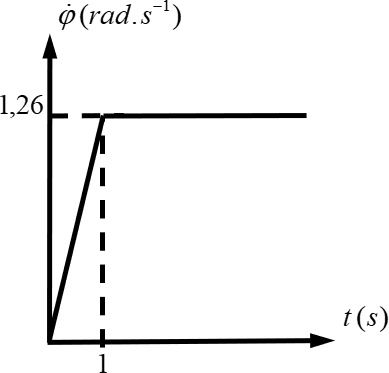
\includegraphics[height=5cm]{img_04}
\caption{Loi de commande de vitesse \label{img:04}}
\end{figure}
\end{minipage} \hfill
\begin{minipage}[b]{.47\linewidth}
\begin{figure}[H]
\centering
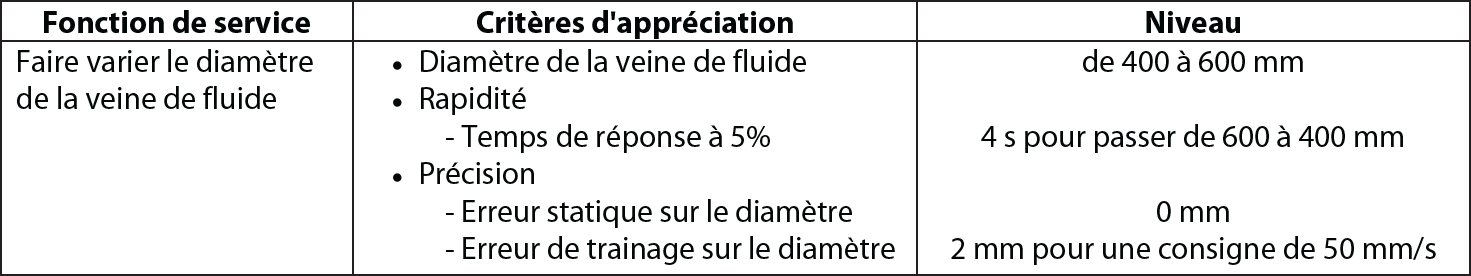
\includegraphics[height=4.5cm]{img_05}

\caption{Paramétrage des roues en contact avec le sol \label{img:05}}
\end{figure}
\end{minipage} 

\vspace{.5cm}

Paramétrage (annexe 9) : 
\begin{itemize}
\item $\rep{0}=\repere{O_0}{x_0}{y_0}{z_0}$ lié au sol \textbf{0} et supposé << galiléen >>;
\item $\rep{L}=\repere{C_1}{x_L}{y_L}{z_L}$ lié à la plateforme PF tel que $\varphi=\angl{x_0}{x_L}=\angl{y_0}{y_L}$ appelé angle de lacet ;
\item $\rep{1}=\repere{C_1}{x_1}{y_1}{z_1}$ lié au pode central \textbf{1} tel que $\beta=\angl{y_L}{y_1}=\angl{z_L}{z_1}$; $\beta$ est l'angle de tangage, $\beta=2\degres$ (supposé constant pendant tout le mouvement du lacet);
\item $\rep{3}=\repere{C_3}{x_3}{y_3}{z_3}$ lié au pode avant \textbf{3} tel que $2\beta=\angl{y_L}{y_3}=\angl{z_L}{z_3}=4\degres$;
\item $\vect{C_1C_3}=b\vect{y_3}$ et $\vect{C_1C_2}=-b\vect{y_L}$ avec $b = \SI{553}{mm}$ ;
\item la \autoref{img:05} permet de définir le paramétrage de chacune des roues de la plate-forme en contact avec le sol avec
l’exemple de la roue centrale droite $R_{1d}$.
\end{itemize}




\begin{tabular}{lccccc}
\hline
&                & Centre          & Point de contact& Vitesse de rotation &  Repère associé \\
&    Nom     & de gravité    & avec le sol &  / au pode central & \\
\hline
\textbf{Roue centrale droite} & $R_{1d}$ & $C_{1d}$ & $I_{1d}$ & $\dot{\theta}_{1d}$ & $\rep{1d}=\repere{C_{1d}}{x_L}{y_{1d}}{z_{1d}}$ \\ 
\textbf{Roue centrale gauche} & $R_{1g}$ & $C_{1g}$ & $I_{1g}$ & $\dot{\theta}_{1g}$ & $\rep{1g}=\repere{C_{1g}}{x_L}{y_{1g}}{z_{1g}}$ \\ 
\textbf{Roue arrière droite} & $R_{2d}$ & $C_{2d}$ & $I_{2d}$ & nulle &  \\ 
\textbf{Roue arrière gauche} & $R_{2g}$ & $C_{2g}$ & $I_{2g}$ & nulle &\\ \hline
\end{tabular}

\fi

\subsection*{Caractéristiques géométriques et d’inertie des solides}
\ifprof
\else

\begin{itemize}
\item Le mouvement de roulis étant nul et le mouvement de tangage étant fixé à une valeur constante, il est possible de définir l’ensemble rigide $\Sigma$ constitué des trois podes \textbf{1}, \textbf{2} et \textbf{3}, des deux roues avant, des deux roues arrière et des bras d’articulation \textbf{4} et \textbf{4’}. Pour chaque constituant de cet ensemble, la masse est supposée répartie uniformément.
\end{itemize}

\begin{center}
\begin{tabular}{|p{4cm}|p{4cm}|p{8cm}|}
\hline
Centre de gravité de $\Sigma$ 
$G$ tel que $\vect{C_1G}=a_G\vect{z_1}$
$a_G =\SI{85}{mm}$
& 
Masse de $\Sigma$ $m_{\Sigma}=\SI{152}{kg}$
& 
Matrice d'inertie de $\Sigma$ en $C_1$ 

$\inertie{C_1}{\Sigma}=
\begin{pmatrix} 
A & 0 & 0 \\ 0 & B & 0 \\ 0 & 0 & C 
\end{pmatrix}_{\base{x_1}{y_1}{z_1}}
\quad 
\begin{array}{l}
A =\SI{30,2}{kg.m^2} \\
B =\SI{8,2}{kg.m^2} \\
C =\SI{32,3}{kg.m^2} \\
\end{array}$ \\
\hline
\end{tabular}
\end{center}


\begin{itemize}
\item Roue droite ou gauche + axe de roue : $R_{\text{i d ou g}}$ ($i$ correspond au numéro du pode).
\end{itemize}

\begin{center}
\begin{tabular}{|p{4cm}|p{4cm}|p{8cm}|}
\hline
Centre de gravité de $R_{\text{i d ou g}}$ $C_{\text{i d ou g}}$ tel que l'entraxe

$C_{ig}=C_{id}=2e$ 

$\vect{C_i C_{id}}=e\vect{x_L}$ et 

$\vect{C_i C_{ig}}=-e\vect{x_L}$ 

$e=\SI{340}{mm}$ 
&
Masse de $R_{\text{i d ou g}}$ $m_r = \SI{4}{kg}$
Rayon d'une roue $R=\SI{225}{mm}$
& 
Matrice d'inertie de $R_{\text{i d ou g}}$ respectivement en  $C_{\text{i d ou g}}$ 

$\inertie{C_{\text{i d ou g}}}{R_{\text{i d ou g}}}=
\begin{pmatrix} 
A_r & 0 & 0 \\ 0 & B_r & 0 \\ 0 & 0 & B_r 
\end{pmatrix}_{\base{x_L}{-}{-}}$

Valable dans toute base orthonormée directe qui contient $\vect{x_L}$
$
\begin{array}{l}
A_r =\SI{0,1}{kg.m^2} \\
B_r =\SI{0,04}{kg.m^2} \\
\end{array}$\\
\hline
\end{tabular}
\end{center}

\begin{itemize}
\item Axe des moteurs du pode central.
\end{itemize}

Les deux motoréducteurs centraux sont constitués chacun d’un moteur à courant continu alimenté en \SI{48}{V} associé à
un réducteur épicycloïdal de rapport de réduction $k = +1/ 25$. La matrice d’inertie en $C_1$ d’un axe moteur droit $M_{1d}$ ou
gauche $M_{1g}$  (en rotation suivant $\axe{C_1}{x_L}$) est :

$\inertie{C_1}{M_{\text{i d}} \text{ ou } M_{\text{i g}}}=
\begin{pmatrix} 
A_m & 0 & 0 \\ 0 & B_m & 0 \\ 0 & 0 & B_m 
\end{pmatrix}_{\base{x_L}{-}{-}}$
avec 
$\begin{array}{l}
A_m =\SI{795e-7}{kg.m^2} \\
B_m =\SI{8e-3}{kg.m^2} \\
\end{array}$.

\begin{itemize}
\item Les masses et inerties des autres pièces seront négligées.
\end{itemize}
\fi
\subsection*{Modélisation du contact roue / sol}
\ifprof
\else

\begin{itemize}
\item Les roues centrales $R_{id}$ et $R_{ig}$ sont motrices, elles roulent sans glisser aux points de contact $I_{1d}$ et $I_{1g}$. On pose $\vect{C_{1d}I_{1d}}=-R\vect{z_L}$ et $\vect{C_{1g}I_{1g}}=-R\vect{z_L}$. Le contact avec le sol \textbf{0} est modélisé par le torseur suivant :

$\torseurstat{T}{0}{R_{1d}}=\torseurl{\vectf{0}{R_{1d}}=Y_{1d}\vect{y_L}+Z_{1d}\vect{z_L}}{\vect{0}}{I_{1d}}$
et
$\torseurstat{T}{0}{R_{1g}}=\torseurl{\vectf{0}{R_{1g}}=Y_{1g}\vect{y_L}+Z_{1g}\vect{z_L}}{\vect{0}}{I_{1g}}$.

\item Les roues arrière $R_{2d}$ et $R_{2g}$ sont bloquées, leur vitesse de rotation par rapport au pode arrière \textbf{2} est nulle. Le contact avec le sol \textbf{0} est modélisé par le torseur suivant : 
$\torseurstat{T}{0}{R_{2d}}=\torseurl{\vectf{0}{R_{2d}}=T_{2d}\vect{n_d}+Z_{2d}\vect{z_L}}{\vect{0}}{I_{2d}}$
et
$\torseurstat{T}{0}{R_{2g}}=\torseurl{\vectf{0}{R_{2g}}=Y_{2g}\vect{n_g}+Z_{2g}\vect{z_L}}{\vect{0}}{I_{2g}}$
avec $\vect{n_d}$ $\vect{n_g}$ deux vecteurs unitaires opposés aux vitesses de glissement des roues $R_{2d}$ et $R_{2g}$ par rapport au sol \textbf{0}
respectivement en $I_{2d}$ et $I_{2g}$. On pose $\vect{C_{2d}I_{2d}}=-R\vect{z_L}$ et 
$\vect{C_{2g}I_{2g}}=-R\vect{z_L}$. $T_{2d}=fZ_{2d}$ et $T_{2g}=fZ_{2g}$; $f$ est le facteur de frottement constant au contact roue/sol; $f = 0,6$.
\end{itemize}
\fi

\subsection*{Autres liaisons}
Toutes les autres liaisons de la plate-forme sont supposées parfaites (sans jeu, sans frottement).

\subsection*{Motoréducteur centraux}
\ifprof
\else

\begin{itemize}
\item L'action mécanique développée par la motoréducteur sur la roue centrale droite $R_{1d}$ est notée : 
$\torseurstat{T}{\text{moteur}}{R_{1d}} = \torseurl{\vect{0}}{-C_m\vect{x_L}}{C_1}$.
\item L'action mécanique développée par la motoréducteur sur la roue centrale gauche $R_{1g}$ est notée : 
$\torseurstat{T}{\text{moteur}}{R_{1g}} = \torseurl{\vect{0}}{C_m\vect{x_L}}{C_1}$.
\end{itemize}
\fi

\question{\label{q_10}Justifier la forme de la matrice d’inertie de l’ensemble $\Sigma$ au point $C_1$ dans la base $\base{x_1}{y_1}{z_1}$.}
\ifprof
\begin{corrige}
Si on considère que les plans  $\left(C_1,\vect{y_1},\vect{z_1}\right)$ et 
$\left(C_1,\vect{z_1},\vect{x_1}\right)$ sont des plans de symétrie, alors $\inertie{\Sigma}{C_1}$ est diagonale.
\end{corrige}
\else
\fi


\ifprof
\else
Dans un premier temps, l’objectif est de déterminer la somme des efforts normaux $Z_{2d}+Z_{2g}$ s’exerçant sur les roues
arrière. Isolons l’ensemble de la plate-forme PF , soit l’ensemble $\Sigma$ , les roues centrales et les motoréducteurs.
Plaçons nous dans le plan médian $\left(C_1;\vect{y_L};\vect{z_L}\right)$ de la plate-forme PF. Nous définissons le projeté $I_1$ des points de contact $I_{1d}$ et $I_{1g}$ dans ce plan. $I_1$ est défini par le vecteur : $\vect{C_1I_1}=-R\vect{z_L}$. 
D’autre part, nous avons 
$\vect{C_2I_1} = b\vect{y_L}-R\vect{z_L}$
$\vect{C_3I_1} = -b\vect{y_3}-R\vect{z_L}$.
Nous ferons l’hypothèse que le moment dynamique $\vectmd{I_1}{PF}{0}\cdot \vect{x_L}$
est négligeable devant les actions mécaniques.

\fi

\question{\label{q_11}En appliquant le théorème du moment dynamique à la plate-forme PF en mouvement par rapport au référentiel galiléen $R_0$ en $I_1$ en projection sur $\vect{x_L}$, déterminer l’expression littérale de la somme des efforts normaux de contact $Z_{2d}+Z_{2g}$, entre les roues arrière et le sol. Réaliser l’application numérique et comparer la valeur obtenue à la somme des efforts normaux s’exerçant sur les roues arrière lorsque la plateforme est immobile en appui sur ses six roues sur un sol plan, à savoir $\left(Z_{2d}+Z_{2g}\right)_{\text{Repos}} = \left(m_2+2m_r\right)g$ avec $m_2=\SI{52}{kg}$ la masse du pode arrière \textbf{2}.}
\ifprof
\begin{corrige}~\\
\begin{minipage}[c]{.47\linewidth}
\begin{itemize}
\item On isole la plate-forme PF. 
\item Bilan des actions mécaniques extérieures : 
\begin{itemize}
\item liaison sphère-plan en $I_{2g}$ : $\torseurstat{T}{0}{2_g}$ 
$=\torseurl{Y_{2g}\vect{n_g}+Z_{2g}\vect{z_L}}{\vect{0}}{I_{2g}}$

$=\torseurl{Y_{2g}\vect{n_g}+Z_{2g}\vect{z_L}}{\vect{I_1I_{2g}}\wedge \left( Y_{2g}\vect{n_g}+Z_{2g}\vect{z_L} \right)}{I_{1}}$

$=\torseurl{Y_{2g}\vect{n_g}+Z_{2g}\vect{z_L}}{\left(-b\vect{y_L}-e\vect{x_L} \right)\wedge \left( Y_{2g}\vect{\pm y_L}+Z_{2g}\vect{z_L} \right)}{I_{1}}$.

On a donc $\vectm{I_1}{0}{2_g}\cdot \vect{x_L}=\left( \left(-b\vect{y_L}-e\vect{x_L} \right)\wedge \left( Y_{2g}\vect{\pm y_L}+Z_{2g}\vect{z_L} \right)\right) \cdot \vect{x_L}$

$= \left(-b\vect{y_L}\wedge \left( Y_{2g}\vect{\pm y_L}+Z_{2g}\vect{z_L} \right)-e\vect{x_L} \wedge \left( Y_{2g}\vect{\pm y_L}+Z_{2g}\vect{z_L} \right)\right) \cdot \vect{x_L}$

$= \left(-b\vect{y_L}\wedge  Z_{2g}\vect{z_L} \right) \cdot \vect{x_L}$
$= -b Z_{2g}$;

%$=\torseurl{Y_{2g}\vect{n_g}+Z_{2g}\vect{z_L}}{-b\vect{x_L} \left( Y_{2g}+Z_{2g} \right)+e \vect{y_L}\left( Y_{2g}+Z_{2g} \right)}{I_{1}}$. On a donc $\vectm{I_1}{0}{2_g}\cdot \vect{x_L}=-b\left( Y_{2g}+Z_{2g} \right)$;
\item liaison sphère-plan en $I_{2d}$ :
 $\vectm{I_1}{0}{2_d}\cdot \vect{x_L}=-bZ_{2d} $;
\item liaison sphère-plan en $I_{1g}$ :
 $\vectm{I_1}{0}{2_d}\cdot \vect{x_L}=0$;
  \item liaison sphère-plan en $I_{2d}$ :
 $\vectm{I_1}{0}{2_d}\cdot \vect{x_L}=0$.
\end{itemize}
\end{itemize}
\end{minipage} \hfill
\begin{minipage}[c]{.47\linewidth}
\begin{figure}[H]
\centering
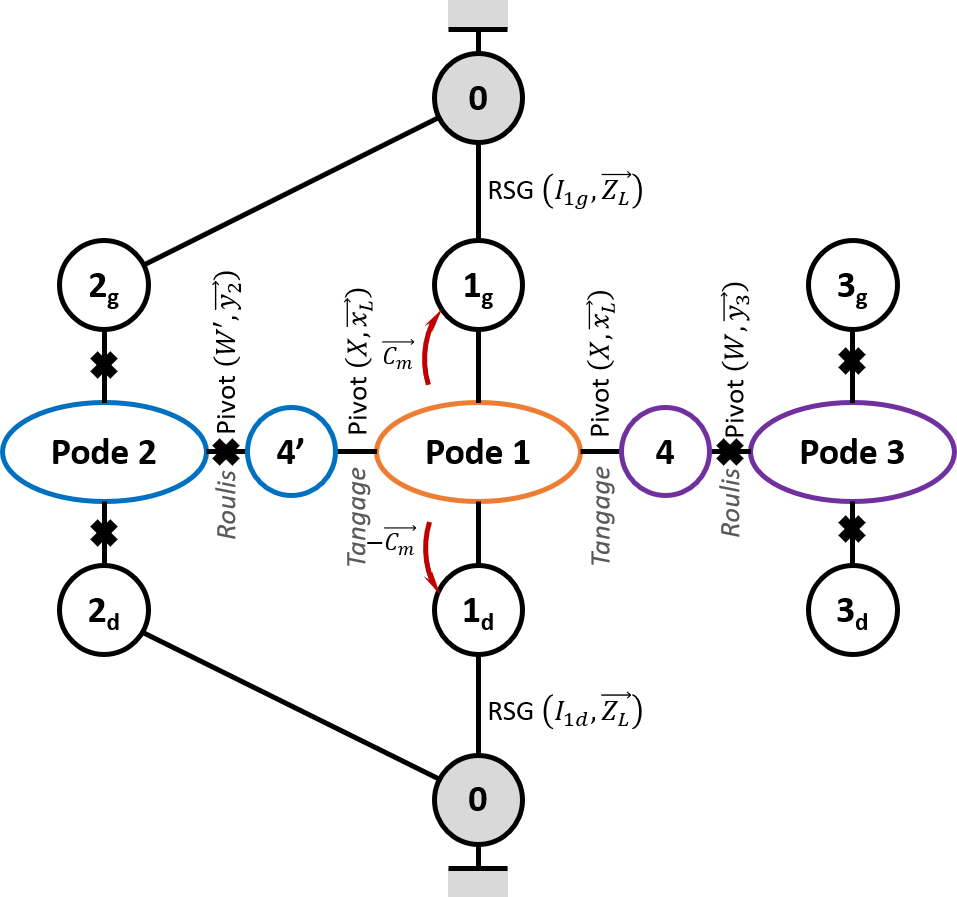
\includegraphics[width=\linewidth]{cor_q11}
\end{figure}
\end{minipage}

\begin{itemize}
\item $\quad$
\begin{itemize}
%\item pesanteur sur la roue $2_g$ :  $\vectm{I_1}{\text{Pes}}{2_g}\cdot \vect{x_L}$
%$=\left(\left(-b\vect{y_L}-e\vect{x_L}  -R \vect{z_L}   \right) \wedge - m_r g \vect{z_L}\right)\cdot \vect{x_L}$
%$=b m_r g $;
%\item pesanteur sur la roue $2_d$ :  $\vectm{I_1}{\text{Pes}}{2_d}\cdot \vect{x_L}$ $=b m_r g $;
\item pesanteur sur $1_g$, $1_d$ et le pode 1 :  $\vectm{I_1}{\text{Pes}}{1_d+1_g+1}\cdot \vect{x_L}=0$;
\item pesanteur de $\Sigma$ : $\vectm{I_1}{\text{Pes}}{\Sigma}\cdot \vect{x_L}$
$ = \left(\vect{I_1 G} \wedge - m_\Sigma g \vect{z_L}\right) \cdot \vect{x_L}$

$ = \left(\left(R \vect{z_L}+ a_G \vect{z_1}\right) \wedge - m_\Sigma g \vect{z_L}\right) \cdot \vect{x_L}$


$ = a_G  m_\Sigma g \sin \beta$

\end{itemize}
\item le moment dynamique étant négligeable, le TMD appliqué à PF en $I_1$ en projection sur $\vect{x_L}$ s'exprime donc par 
$ a_G  m_\Sigma g \sin \beta -b Z_{2g}-bZ_{2d} =0 $
\end{itemize}

Au final, \fbox{$Z_{2g}+ Z_{2d}= \dfrac{ a_G  m_\Sigma g \sin \beta  }{b} $}.

AN : $Z_{2g}+ Z_{2d}= \dfrac{ 85\times 152 \times  9,81 \times  \sin 2\degres  }{553}=\SI{8}{N} $.
Au repos, $\left(Z_{2d}+Z_{2g}\right)_{\text{Repos}} \simeq \SI{590}{N}$. Dans cette phase, le train arrière (pode 2) est donc soulagé pour faciliter le mouvement. 

\end{corrige}

\else
\fi


L’objectif est dans un second temps de valider l’aptitude des moteurs à suivre la loi de vitesse en lacet exigée. Il est
proposé de déterminer l’expression du couple moteur $C_m$ par une approche énergétique.


\question{\label{q_12}Déterminer l’énergie cinétique galiléenne de l’ensemble des solides en mouvement. Le résultat sera mis
sous la forme $\dfrac{1}{2}J\varphip^2$ où $J$ est à exprimer sous forme littérale en fonction des données du problème.}
\ifprof
\begin{corrige}
On a :
\begin{itemize}
\item $\ec{\Sigma}{0}=\dfrac{1}{2}\torseurci{\Sigma}{0}\otimes \torseurcin{V}{\Sigma}{0}$

$=\dfrac{1}{2}\torseurl{m_{\Sigma}\vectv{G}{\Sigma}{0}}{\vectmc{C_1}{\Sigma}{0}}{C_1}\otimes \torseurl{\vecto{\Sigma}{0}}{\vectv{C_1}{\Sigma}{0}}{C_1}$
$=\dfrac{1}{2}\torseurl{m_{\Sigma}\vectv{G}{\Sigma}{0}}{\vectmc{C_1}{\Sigma}{0}}{C_1}\otimes \torseurl{\vecto{\Sigma}{0}}{\vect{0}}{C_1}$
%\item On a $\vectv{G}{\Sigma}{0} =\vectv{C_1}{\Sigma}{0} + \vect{GC_1}\wedge \vecto{\Sigma}{0}$.
%$ = \vect{0}-a_G \vect{z_1}\wedge \varphip \vect{z_0}$ 
%$ = a_G \varphip  \sin\beta \vect{x_0}$ 
Or,  $\vectmc{C_1}{\Sigma}{0}=\inertie{\Sigma}{C_1}\vecto{\Sigma}{0} + m_{\Sigma} \vect{C_1 G}\wedge\vectv{C_1}{\Sigma}{0} $ $=\inertie{\Sigma}{C_1}\vecto{\Sigma}{0} $
 $=\inertie{\Sigma}{C_1}\varphip \vect{z_0} $ 
 $=\inertie{\Sigma}{C_1}\varphip \left( \cos\beta \vect{z_1}+\sin\beta \vect{y_1}\right) $
  $= C\varphip\cos\beta \vect{z_1}+B\varphip\sin\beta \vect{y_1} $ . 
 
On a donc $\ec{\Sigma}{0} = \dfrac{1}{2}\varphip \left(C\cos\beta \vect{z_1}+B\sin\beta \vect{y_1}\right) \cdot \varphip\left( \cos\beta \vect{z_1}+\sin\beta \vect{y_1}\right)$ 
$= \dfrac{1}{2}\varphip^2 \left(C\cos^2\beta +B\sin^2\beta\right)$ .
\item $\ec{1_g}{0}=\dfrac{1}{2}\torseurci{1_g}{0}\otimes \torseurcin{V}{1_g}{0}$. On a : 
\begin{itemize}
\item $\torseurcin{V}{1_g}{0}$ $=\torseurcin{V}{1_g}{\Sigma}+\torseurcin{V}{\Sigma}{0} $ 
$ = \torseurl{\thetap_{1g}\vect{x_L}}{\vect{0}}{C_{1g}} + \torseurl{\varphip\vect{z_0}}{\vect{0}}{C_{1}}$
$ = \torseurl{\thetap_{1g}\vect{x_L}}{\vect{0}}{C_{1g}}
 + \torseurl{\varphip\vect{z_0}}{\vect{C_{1g}C_1}\wedge \varphip\vect{z_0}}{C_{1g}}$
$ = \torseurl{\thetap_{1g}\vect{x_L}+\varphip\vect{z_0}}{e\vect{x_L}\wedge \varphip\vect{z_0}}{C_{1g}}$
$ = \torseurl{\thetap_{1g}\vect{x_L}+\varphip\vect{z_0}}{-e\varphip\vect{y_L}}{C_{1g}}$
\item $\torseurci{1_g}{0}=\torseurl{m_{r}\vectv{G}{1_g}{0}}{\inertie{1g}{C_{1g}}\vecto{1_g}{0}}{C_{1g}}$ 
$=\torseurl{m_{r}\vectv{C_{1g}}{1_g}{0}}{A_r \thetap_{1g} \vect{x_L}+ B_r \varphip\vect{z_0}  }{C_{1g}}$,
\item $\ec{1_g}{0}= \dfrac{1}{2} \left(m_re^2\varphip^2 + A_r \thetap_{1g}^2 + B_r \varphip^2\right)$. Par ailleurs, $\dot{\thetap}^2 = \dfrac{e^2 \dot{\varphip}^2}{R^2}$. 

On a donc 
$\ec{1_g}{0}= \dfrac{1}{2} \left(m_re^2\varphip^2 + A_r \dfrac{e^2 \dot{\varphip}^2}{R^2} + B_r \varphip^2\right)$
$= \dfrac{1}{2} \varphip^2\left(m_re^2 + A_r \dfrac{e^2}{R^2} + B_r \right)$.
\end{itemize}
\item $\ec{1_d}{0}= \dfrac{1}{2} \varphip^2\left(m_re^2 + A_r \dfrac{e^2}{R^2} + B_r \right)$.

\item $\ec{M1_g}{0}$ à la même forme que $\ec{1_g}{0}$ à ceci près qu'il faut prendre en compte le rapport de réduction du réducteur. On a donc $\ec{M1_g}{0}= \dfrac{1}{2} \varphip^2\left( A_m \dfrac{e^2}{k^2 R^2} + B_m \right)$.
\end{itemize}

Au final, $\ec{\Sigma}{0} =  \varphip^2\left(m_re^2 + A_r \dfrac{e^2}{R^2} + B_r +  A_m \dfrac{e^2}{k^2 R^2} + B_m \right)+\dfrac{1}{2}\varphip^2 \left(C\cos^2\beta +B\sin^2\beta\right)$.

Dans ces conditions, \fbox{$J = 2\left(m_re^2 + A_r \dfrac{e^2}{R^2} + B_r +  A_m \dfrac{e^2}{k^2 R^2} + B_m \right)+\left(C\cos^2\beta +B\sin^2\beta\right)$}.
\end{corrige}
\else
\fi


\question{\label{q_13}Mettre en \oe{}uvre le théorème de l’énergie cinétique afin de déterminer l’expression du couple moteur. Vous
donnerez le résultat sous la forme $C_m = k_2\left( J\varphipp +k_1\left(T_{2d}+T_{2g}\right)\right)$ où $k_1$ et $k_2$ sont à exprimer sous forme littérale en fonction des données du problème.
Vous veillerez à bien faire apparaître les différentes étapes de votre raisonnement et à fournir des expressions littérales.}
\ifprof
\begin{corrige}
En appliquant le théorème de l'énergie cinétique à l'ensemble des solides en mouvement $E$ est donné par 
$$
\deriv{\ec{E}{0}}{}  = \mathcal{P}_{\text{int}}(E)+\pext{\overline{E}}{E}{0}.
$$

\textbf{Bilan des puissances extérieures}
\begin{itemize}
\item Puissance des actions de pesanteur : $\pext{g}{0}{0}=0$ car le mouvement est selon $\vect{x_0}$.
\item Puissance des actions sur $1_g$ et $1_d$ : $\pext{0}{1_g}{0}=\pext{0}{1_d}{0}=0$ (contact ponctuel avec roulement sans glissement).
\item Puissance des actions sur $2_g$ : $\pext{0}{2_g}{0} = \torseurstat{T}{0}{2_g} \otimes\torseurcin{V}{2_g}{0}$ 

$=\torseurl{T_{2g}\vect{n_g}+Z_{2g}\vect{z_L}}{\vect{0}}{I_{2g}} \otimes \torseurl{*}{\vectv{I_{2g}}{2_g}{0}}{I_{2g}}$. On a alors 
$\vectv{I_{2g}}{2_g}{0}=\underbrace{\vectv{I_{2g}}{2_g}{PF}}_{\vect{0}}+\vectv{I_{2g}}{PF}{0}$ 
$=\vectv{C_1}{PF}{0} + \vect{I_{2g} C}\wedge \varphip \vect{z_0}$
$= \left(R\vect{z_L}  +b\vect{y_L} +e\vect{x_L}\right)\wedge \varphip \vect{z_0}$
$= b\varphip \vect{x_L} - e \varphip \vect{y_L}$.

Au final, $\pext{0}{2_g}{0} = \left( -T_{2g}\vect{x_L}+Z_{2g}\vect{z_L} \right) \cdot\left( b\varphip \vect{x_L} - e \varphip \vect{y_L}\right)$
$ = -T_{2g}\vect{x_L}\cdot\left( b\varphip \vect{x_L} - e \varphip \vect{y_L}\right)+Z_{2g}\vect{z_L} \cdot\left( b\varphip \vect{x_L} - e \varphip \vect{y_L}\right) $
$ = -T_{2g} b\varphip $

\item Puissance des actions sur $2_d$ : $\pext{0}{2_d}{0}= -T_{2d} b\varphip $
\end{itemize}

\textbf{Bilan des puissances intérieures}
\begin{itemize}
\item Puissance des moteurs : $\mathcal{P}_{\text{mot}} = 2 C_m \dfrac{e}{kR}\varphip$.
\end{itemize}

Au final, 
$J\varphip\varphipp = 2 C_m \dfrac{e}{kR}\varphip -T_{2d} b\varphip-T_{2g} b\varphip$
soit 
$  C_m  =\dfrac{kR}{2e} \left(J\varphipp  +T_{2d} b+T_{2g} b\right) $

\end{corrige}
\else
\fi



Pour la question \ref{q_14}, vous prendrez $J =\SI{34}{kg.m^2}$, $k_1 =\SI{0,65}{m}$ et $k_2 = \num{1,3e-2}$.

\question{\label{q_14} Calculer le couple moteur maximal : $C_m$ maxi. À partir du graphe de fonctionnement du moteur (figure \ref{rep_q14}), conclure quand à l’aptitude de la motorisation à générer le mouvement de lacet désiré.}
\ifprof
\begin{corrige}
D'une part : $  C_m  =\dfrac{kR}{2e} \left(J\varphipp  +b\left( T_{2d} +T_{2g} \right)\right) $ 
$=k_2 \left(J\varphipp  +k_1\left( T_{2d} +T_{2g} \right)\right) $.

D'autre part : $Z_{2g}+ Z_{2d}= \dfrac{ a_G  m_\Sigma g \sin \beta  }{b} $.

Enfin en utilisant les lois de Coulomb, on a $\left( T_{2d} +T_{2g} \right) = f\left( Z_{2d} +Z_{2g} \right)$.

On a donc, $  C_m  =k_2 \left(J\varphipp  +k_1f\dfrac{ a_G  m_\Sigma g \sin \beta  }{b}\right) $.

D'après la loi de commande $\varphipp = \SI{1,26}{rad.s^{-2}}$
et donc $C_m = 1,3\times 10^{-2}\left(34\times 1,26 + 0,65 \times 0,6 \dfrac{ 85 \times 152 \times  9,81 \times  \sin 2 }{553}\right) \simeq \SI{1,6}{Nm}$.

\end{corrige}
\else
\fi

\begin{figure}[H]
\centering
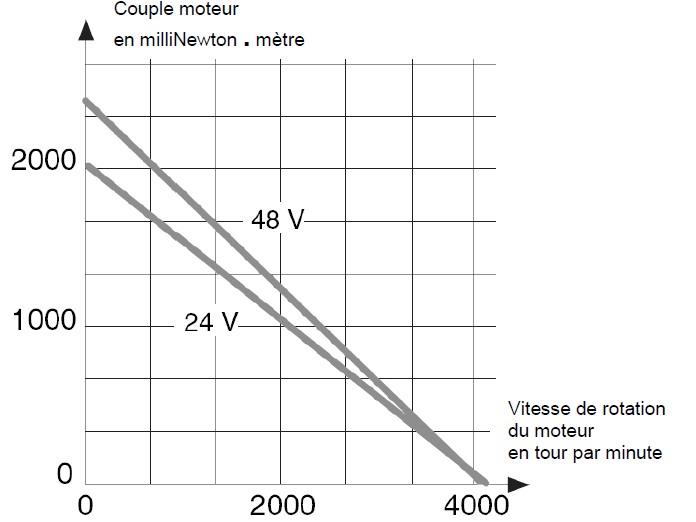
\includegraphics[width=.6\linewidth]{rep_q14}
\caption{Graphe de fonctionnement du moteur\label{rep_q14}}
\end{figure}



%\section{Fonction technique FT2 : gérer le fonctionnement}
\section{Exigence fonctionnelle ID 1.2 : gérer le fonctionnement}
\subsection{La commande de la plate-forme}

\ifprof
\else

Pour coordonner les déplacements, la plate-forme est équipée de deux parties commandes supportées par deux microcontrôleurs placés respectivement dans les podes avant et arrière (\autoref{img:06}).

\begin{figure}[H]
\centering
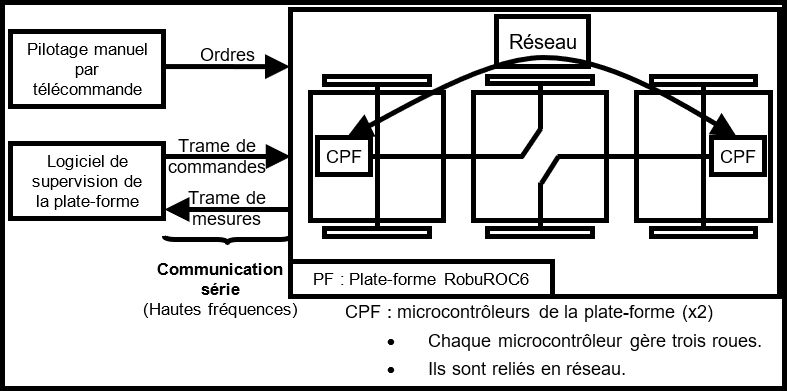
\includegraphics[width=.7\linewidth]{img_06}
\caption{Loi de commande de vitesse \label{img:06}}
\end{figure}

Chaque microcontrôleur commande trois roues et l’un des deux génère les ordres envoyés à la centrale hydraulique afin de piloter les mouvements de tangage. Ces 2 microcontrôleurs communiquent entre eux et dialoguent avec l’extérieur suivant deux modes de conduite :
\begin{itemize}
\item le mode joystick : l’utilisateur pilote manuellement la plate-forme par l’intermédiaire d’une télécommande ;
\item le mode automatique : la plate-forme traite les commandes du logiciel de supervision.
\end{itemize}
Le pilotage en mode automatique est prioritaire sur le mode joystick. 
Les principales fonctions à remplir par la partie commande sont :
\begin{itemize}
\item communiquer avec l’utilisateur ou le superviseur ;
\item gérer les séquences de pilotage, notamment celle de cabrage ;
\item asservir les déplacements de la plate-forme.
\end{itemize}
\fi

\subsection{Gérer le pilotage séquentiel du CABRAGE en << Mode 2 roues instable >>}

\ifprof
\else

Lorsque le rayon de courbure est inférieur à 4 mètres et que la vitesse de la plate-forme est inférieure à une vitesse
limite, la partie commande de la plate-forme active le << Mode 2 roues instable >> (Rotation 2 roues=1). En << Mode 2 roues instable >>, la partie commande génère les lois de pilotage à appliquer aux roues centrales et pilote la centrale hydraulique afin de CABRER les podes avant et arrière suivant une séquence prédéfinie.
L’objectif de cette partie est de proposer un GRAFCET de gestion de la
séquence CABRAGE en << Mode 2 roues instable >>. La table des
entrées-sorties de cette séquence est la suivante.

\begin{figure}[H]
\centering
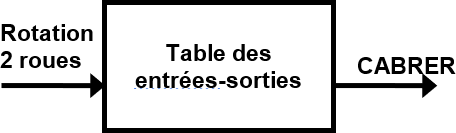
\includegraphics[width=.3\linewidth]{img_06_2}
\caption{Loi de commande de vitesse \label{img:06:2}}
\end{figure}

\textbf{Description de la séquence associée au CABRAGE en « Mode 2 roues instable »}

\begin{enumerate}
\item Lorsque Rotation 2 roues=1, une consigne CABRER est envoyée à la centrale hydraulique pendant 1 seconde (temps nécessaire pour imposer un angle de tangage de l’ordre de 2\ieme aux podes avant et arrière par rapport au pode central).
\item Le système hydraulique actuel ne permet pas de bloquer en permanence les podes avant et arrière en position CABRER. En effet, les pressions importantes présentes dans le circuit pour maintenir les podes en position génèrent un débit de fuite interne qui ramène progressivement les podes en position initiale. Il a été mesuré qu’au bout de 5 secondes (temps nécessaire pour effectuer de 1 à 2 tours sur place en fonction de la nature du sol), les podes avant et arrière sont à nouveau pleinement en contact avec le sol.
\item Si le « Mode 2 roues instable » (Rotation 2 roues=1) est maintenu pendant plus de 5 secondes (à partir de son activation) alors la séquence prévoit de rétablir à nouveau la consigne CABRER (retour à l’étape 1).
\item À tout moment, le « Mode 2 roues instable~» peut être désactivé (Rotation 2 roues=0). Si une consigne CABRER est en cours, elle est immédiatement arrêtée et la séquence de gestion de la centrale hydraulique en «~Mode 2 roues instable~» est réinitialisée. Le débit de fuite dans le circuit assure le retour progressif en
position initiale des podes avant et arrière.
\end{enumerate}
\fi

%\question{\label{q_15}Réaliser un (ou plusieurs) GRAFCET(s) correspondant à la séquence de fonctionnement associée au CABRAGE en «~Mode 2 roues instable~». Un début de GRAFCET est fourni sur le document-réponse
%(question \ref{q_15}). Vous veillerez en particulier à :}
%\textit{
%\begin{itemize}
%\item respecter les normes de construction d’un GRAFCET ;
%\item utiliser uniquement les entrées-sorties fournies ;
%\item mettre en place les temporisations nécessaires ;
%\item ajouter des commentaires aux étapes qui ne pilotent pas directement une action afin de définir leur rôle.
%\end{itemize}}
%\ifprof
%\begin{corrige}
%\end{corrige}
%\else
%\fi

\question{\label{q_15} Compléter le STM (diagramme d'états) correspondant à la séquence de fonctionnement associée au
CABRAGE en «Mode 2 roues instable ». Un diagramme d'états est fourni sur le document-réponse
(question \ref{q_15}). Vous veillerez en particulier à :
\begin{itemize}
\item compléter les deux événements 1 et 2 permettant l'entrée et la sortie dans "Mode 2 roues instable";
\item compléter les deux événements 3 et 4 (si nécessaire);
\item compléter les actions (5 et éventuellement 6) réalisées (vous pouvez utiliser Entry et/ou Do);
\item sule la compréhension du fonctionnement sera évaluée. Le respect de la norme ne sera pas pris en compte. Vous écrirez les événements sous la forme de conditions booléennes.
\end{itemize}}

\ifprof
\begin{corrige}
\end{corrige}
\else
\fi


\subsection{Asservir les déplacements de la plate-forme}
\ifprof
\else

Les déplacements de la plate-forme sont contrôlés de la manière suivante :
\begin{itemize}
\item au niveau de chacun des 6 moteurs, des boucles de vitesse assurent l’asservissement dit « bas niveau » ;
\item à partir d’informations sur la position absolue de la plate-forme via le système GPS par exemple, un asservissement en position de la plate-forme peut être mis en place (asservissement dit « haut niveau »).
\end{itemize}
L’objectif dans cette partie est de déterminer les paramètres de réglage de chacune des boucles d’asservissement en vitesse de la plate-forme par rapport au sol.

\begin{hypo}
Afin de régler l’asservissement en vitesse de la plate-forme par rapport au sol :
\begin{itemize}
\item un déplacement en ligne droite de la plate-forme est considéré (consigne de vitesse $V_C(t)$, les paramètres
angulaires de lacet, tangage et roulis restent nuls) ;
\item le contact entre chaque pneumatique et le sol est considéré avec roulement sans glissement ;
\item pour la modélisation du fonctionnement des moteurs, nous supposerons une équi-répartition de la charge extérieure sur chacun des six moteurs. Ainsi, pour une vitesse $V (t)$ de la plate-forme, les six moteurs tourneront à la même vitesse $\Omega_{\text{Mot}}(t)$. Ils seront alimentés par une même tension de commande $U(t)$ et devront fournir un même couple moteur $C_{\text{Mot}}(t)$ ;
\item les efforts de perturbations (action mécanique de la pesanteur sur une pente…) seront répartis sur chacun des axes des six moteurs et seront donc modélisés par un même couple de perturbation équivalent $C_{\text{equ}}(t)$ appliqué sur chacun des axes moteurs ;
\item les caractéristiques inertielles de la plate-forme seront représentées au niveau de chaque axe moteur par un moment d’inertie équivalent $\dfrac{J_{\text{equ}}}{6}$;
\item le comportement individuel d’un des six moteurs peut donc être approché par celui d’un moteur à courant continu avec les équations électromécaniques suivantes :
\begin{itemize}
\item équation électrique : $U(t)=E(t)+RI(t)+L\dfrac{\dd i(t)}{\dd t}$,
\item équation mécanique : $\dfrac{J_{\text{eq}}}{6} \dfrac{\dd \Omega_{\text{Mot}}(t)}{\dd t} = C_{\text{Mot}}(t)-C_{\text{equ}}(t)$,
\item équation de couplage $E(t)=k_e\Omega_{\text{Mot}}(t)$ et $C_{\text{Mot}}(t) = k_c I(t)$.
\end{itemize}
\end{itemize}
\end{hypo}



\begin{center}
\begin{tabular}{lll}
\hline
\textbf{Symbole} & \textbf{Désignation} & \textbf{Valeur, unités} \\  \hline
$U(t)$  			& Tension d’alimentation d’un moteur 		& $\si{V}$ \\ 
$E(t)$ 			& Tension contre électromotrice dans un moteur 	& $\si{V}$ \\ 
$I (t)$			& Intensité dans un moteur 			& $\si{A}$ \\ 
$V(t)$ 			& Vitesse de déplacement de la plate-forme 		& $\si{m/s}$\\ 
$\Omega_{\text{Mot}}(t)$& Vitesse de rotation de chacun des six moteurs	& $\si{rad/s}$ \\
$C_{\text{Mot}}(t)$ 	& Couple moteur appliqué par chacun des six moteurs & $\si{Nm}$ \\ 
$C_{\text{equ}}(t)$ 	& Couple de perturbation équivalent appliqué à chacun des six axes moteurs
& $\si{Nm}$ \\ 
$r$ 			& Résistance de l’induit d’un moteur 		& $\SI{2,2}{\Omega}$ \\ 
$L$ 			& Inductance de l’induit d’un moteur 	& $\SI{4,62}{mH}$ \\ 
$k_e$ 			& Constante de vitesse d’un moteur 	& $\SI{0,12}{V/(rad/s)}$ \\ 
$k_c$ 			& Constante de couple d’un moteur 		& $\SI{0,12}{Nm/A}$ \\ 
$J_{\text{equ}}$		& Inertie équivalente de la plate-forme ramenée sur l’axe d’un des six moteurs
& $\SI{14,4e-3}{kg.m^2}$ \\ \hline
\end{tabular}
\end{center}

\textbf{Description de l’asservissement en vitesse de la plate-forme par rapport au sol (\autoref{img:07} et \autoref{img:08})}

Pour une vitesse de consigne $V_C (t)$ en \si{m/s}, les microcontrôleurs de pilotage génèrent une vitesse de rotation de consigne à appliquer à chaque moteur $\Omega_{\text{C Mot}}(t)$ \si{rad/s} qui est convertie en une tension de consigne $U_C (t)$ en \si{V}. Un capteur de vitesse monté sur l’axe de chaque moteur fournit une tension mesurée $U_m (t)$ en \si{V}, image de la vitesse de rotation réelle $\Omega_{\text{Mot}}(t)$. Un correcteur (défini par la suite) adapte le signal écart entre la tension de consigne et la tension mesurée, ce qui permet après amplification de définir la tension d’alimentation $U(t)$ à appliquer aux moteurs. La vitesse réelle de la plate-forme $V (t)$ est déterminée à partir de $\Omega_{\text{Mot}}(t)$ en l’absence de glissement.

\begin{figure}[H]
\centering
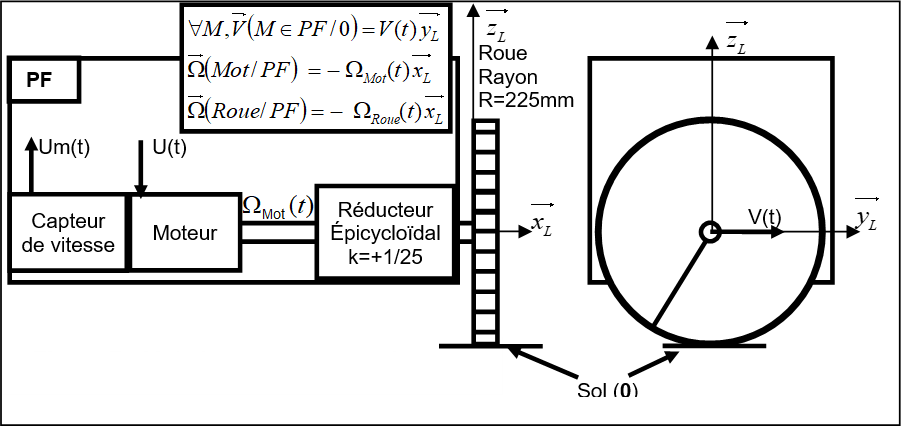
\includegraphics[width=.8\linewidth]{img_07}
\caption{Motorisation d'un des six roues\label{img:07}}
\end{figure}

\begin{figure}[H]
\centering
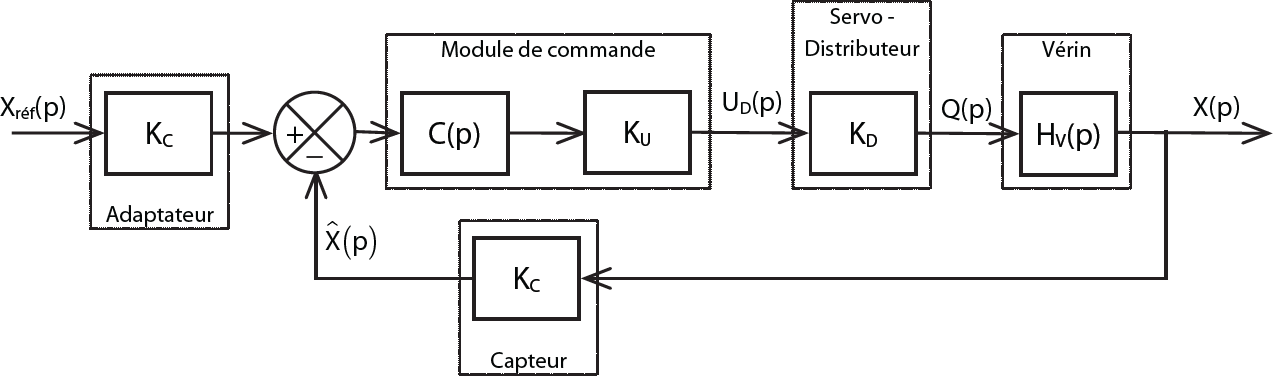
\includegraphics[width=\linewidth]{img_08}
\caption{Schéma-blocs fonctionnel de l’asservissement en vitesse d’un des six moteurs\label{img:08}}
\end{figure}


\begin{figure}[H]
\centering
\begin{tabular}{lc}
\hline
\textbf{Blocs} & \textbf{Fonctions de transfert} 	\\ \hline
Générateur de consigne 	& $K_G$ (à déterminer) 		\\ 
Convertisseur 		& $K_{\text{conv}}$(à déterminer)	\\ 
Correcteur 		& $C(p)$ (réglé par la suite)	\\ 
Amplificateur 		& $K_A = 20 $ (sans unité)	\\ 
Capteur de vitesse 	& $K_{\text{Capt}}= \SI{5e-3}{V/(rad/s)}$ 	\\ 
Rapport cinématique 	& $K_R$ (à déterminer) 	\\ \hline
\end{tabular}

\caption{Schéma-blocs fonctionnel de l’asservissement en vitesse d’un des six moteurs\label{img:09}}
\end{figure}

\textbf{Cahier des charges à respecter}

\begin{center}
\begin{tabular}{lp{9cm}l}
\hline
\textbf{Fonction} & \textbf{Critères} & \textbf{Niveaux} \\ \hline\hline
\multirow{7}{3cm}{Asservir en vitesse la plateforme par rapport au sol} & 
Stabilité & \\ %\cline{2-3}
& Marge de gain		& $M_G=\SI{6}{dB}$ mini \\ %\cline{2-3}
& Marge de phase	& $M_{\varphi} =45\degres$ mini \\ \cline{2-3}
& Précision en poursuite : écart statique à un échelon de vitesse & Nulle \\ %\cline{2-3}
& Précision en régulation : influence d'un échelon en couple de pertubation en régime permanent  & Nulle \\ \cline{2-3}%\hline
& Rapidité : temps de réponse à 5\% (à une entrée en échelon de vitesse) & \SI{0,5}{s} \\ \hline
\end{tabular}
\end{center}
\fi

\question{\label{q_16}Déterminer les valeurs numériques et unités des gains associés au générateur de consigne (noté $K_G$), au rapport cinématique ($K_R$) et au convertisseur ($K_{\text{conv}}$) en sachant, que lorsque la vitesse réelle de la plateforme $V (t)$ est égale à la vitesse de consigne de la plate-forme $V_C (t)$ , l’écart $\varepsilon(t)$ doit être nul.}
\ifprof
\begin{corrige}
\paragraph*{Détermination de $K_G$}
On a $V(t)=R\indice{\Omega}{roue}$ et $\indice{\Omega}{roue} =\indice{\Omega}{Mot}k  \indice{\Omega}{roue}$ et $V(t) = kR \indice{\Omega}{Mot}$. 
On a donc $K_G =  \dfrac{1}{kR}$.


\textit{Application numérique :} $K_G = \dfrac{1}{\dfrac{1}{25}\times 225\times 10^{-3}} = \SI{111}{m}$.

\paragraph*{Détermination de $K_R$}
$K_R =  kR = \SI{0,009}{m^{-1}}$.

\paragraph*{Détermination de $\indice{K}{conv}$}
$\indice{K}{conv}=\indice{K}{Capt}=\SI{5e-3}{V/(rad/s)}$.
\end{corrige}
\else
\fi


\question{\label{q_17} Compléter le schéma-blocs sur le document-réponse (question \ref{q_17}) en y faisant figurer les fonctions de transfert sous forme littérale dans le domaine de Laplace avec des conditions initiales nulles, ainsi que les signes des sommateurs.}
\ifprof
\begin{corrige}
\begin{figure}[H]
\centering
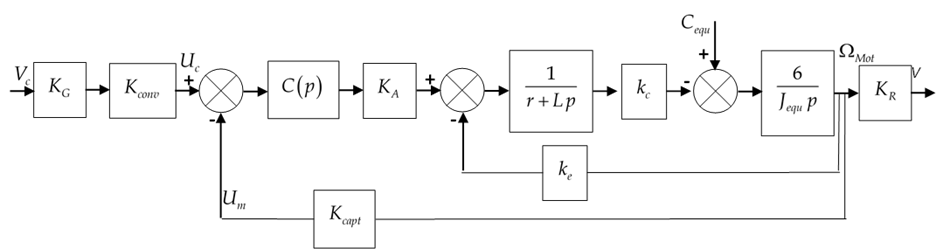
\includegraphics[width=\linewidth]{cor_q17}
%\caption{Schéma-blocs à retour unitaire\label{img:10}}
\end{figure}
\end{corrige}
\else
\begin{figure}[H]
\centering
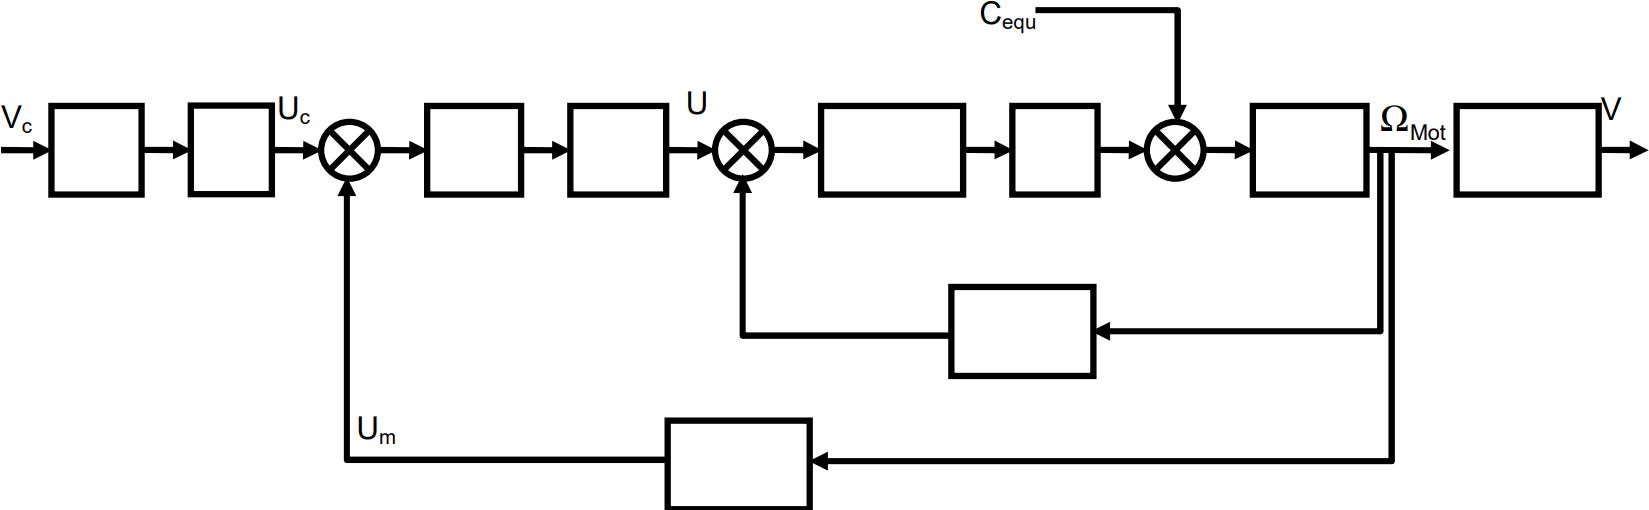
\includegraphics[width=\linewidth]{rep_q17}
\caption{Schéma-blocs à remplir de la question \ref{q_17}}
\end{figure}

\fi


À partir de la modélisation des blocs, un schéma-blocs à retour unitaire est tracé.

\begin{figure}[H]
\centering
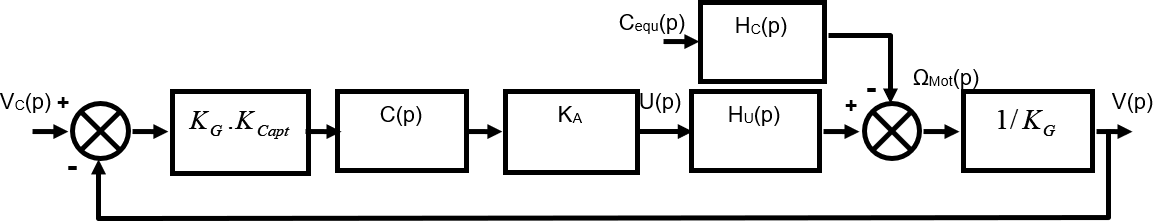
\includegraphics[width=\linewidth]{img_10}
\caption{Schéma-blocs à retour unitaire\label{img:10}}
\end{figure}

$H_U( p)$ et $H_C( p)$ sont les fonctions de transfert caractéristiques d’un des six moteurs. Nous retiendrons :
$H_U(p)=\dfrac{K_U}{\left(T_1p +1\right)\left(T_2p +1\right)}$ et $H_C(p)=\dfrac{K_C\left(\dfrac{L}{r}p +1\right)}{\left(T_1p +1\right)\left(T_2p +1\right)}$
avec 
$K_U = \SI{8,3}{rad . s ^{-1}.V ^{-1}}$, 
$K_C = \SI{152,7}{rad . s^{-1}.N^{-1} .m^{-1}}$, 
$T_1=\SI{2,1}{ms}$, 
et $T_2 =\SI{0,36}{s}$.

\subsubsection{Etude des performances sans correction : $C( p) =1$}
Nous distinguerons dans la suite :
\begin{itemize}
\item l’étude en poursuite : le couple de perturbation équivalent $C_{\text{equ}} (t)$ est nul $V_c (t)$ varie ;
\item l’étude en régulation : la vitesse de consigne de la plate-forme $V_c (t)$ est nulle. $C_{\text{equ}}(t)$ varie.
\end{itemize}

Les diagrammes de Bode de la Fonction de Transfert en Boucle Ouverte $\text{FTBO}( p)$ non corrigée sont fournis sur le document-réponse ou sur la figure \ref{rep_q_18} pour $C( p) = 1$.

\question{Le système étudié est-il stable théoriquement ? Justifier vos réponses.}
\ifprof
\begin{corrige}
La stabilité est indépendante de la perturbation. On peut donc ne pas la prendre en compte ici. 
\begin{itemize}
\item Possibilité 1 : la boucle ouverte est un ordre 2 avec tous les coefficients positifs. En bouclant, on aura encore un ordre 2 avec tous les coefficients positifs. Le système est donc stable. En effet, 
$\indice{H}{BF}(p)=\dfrac{\indice{K}{Capt}K_A\dfrac{K_U}{\left(T_1p +1\right)\left(T_2p +1\right)}}{1+\indice{K}{Capt}K_A\dfrac{K_U}{\left(T_1p +1\right)\left(T_2p +1\right)}}$
$=\dfrac{\indice{K}{Capt}K_AK_U}{\left(T_1p +1\right)\left(T_2p +1\right)+\indice{K}{Capt}K_AK_U}$.
\item Possibilité 2 : d'après le diagramme de Bode de la boucle ouverte, le gain est toujours négatif et la phase toujours supérieure à $-\SI{180}{\degres}$. D'après le critère du Revers, le système est stable.  
\end{itemize}
\end{corrige}
\else

\begin{figure}[t]
\centering
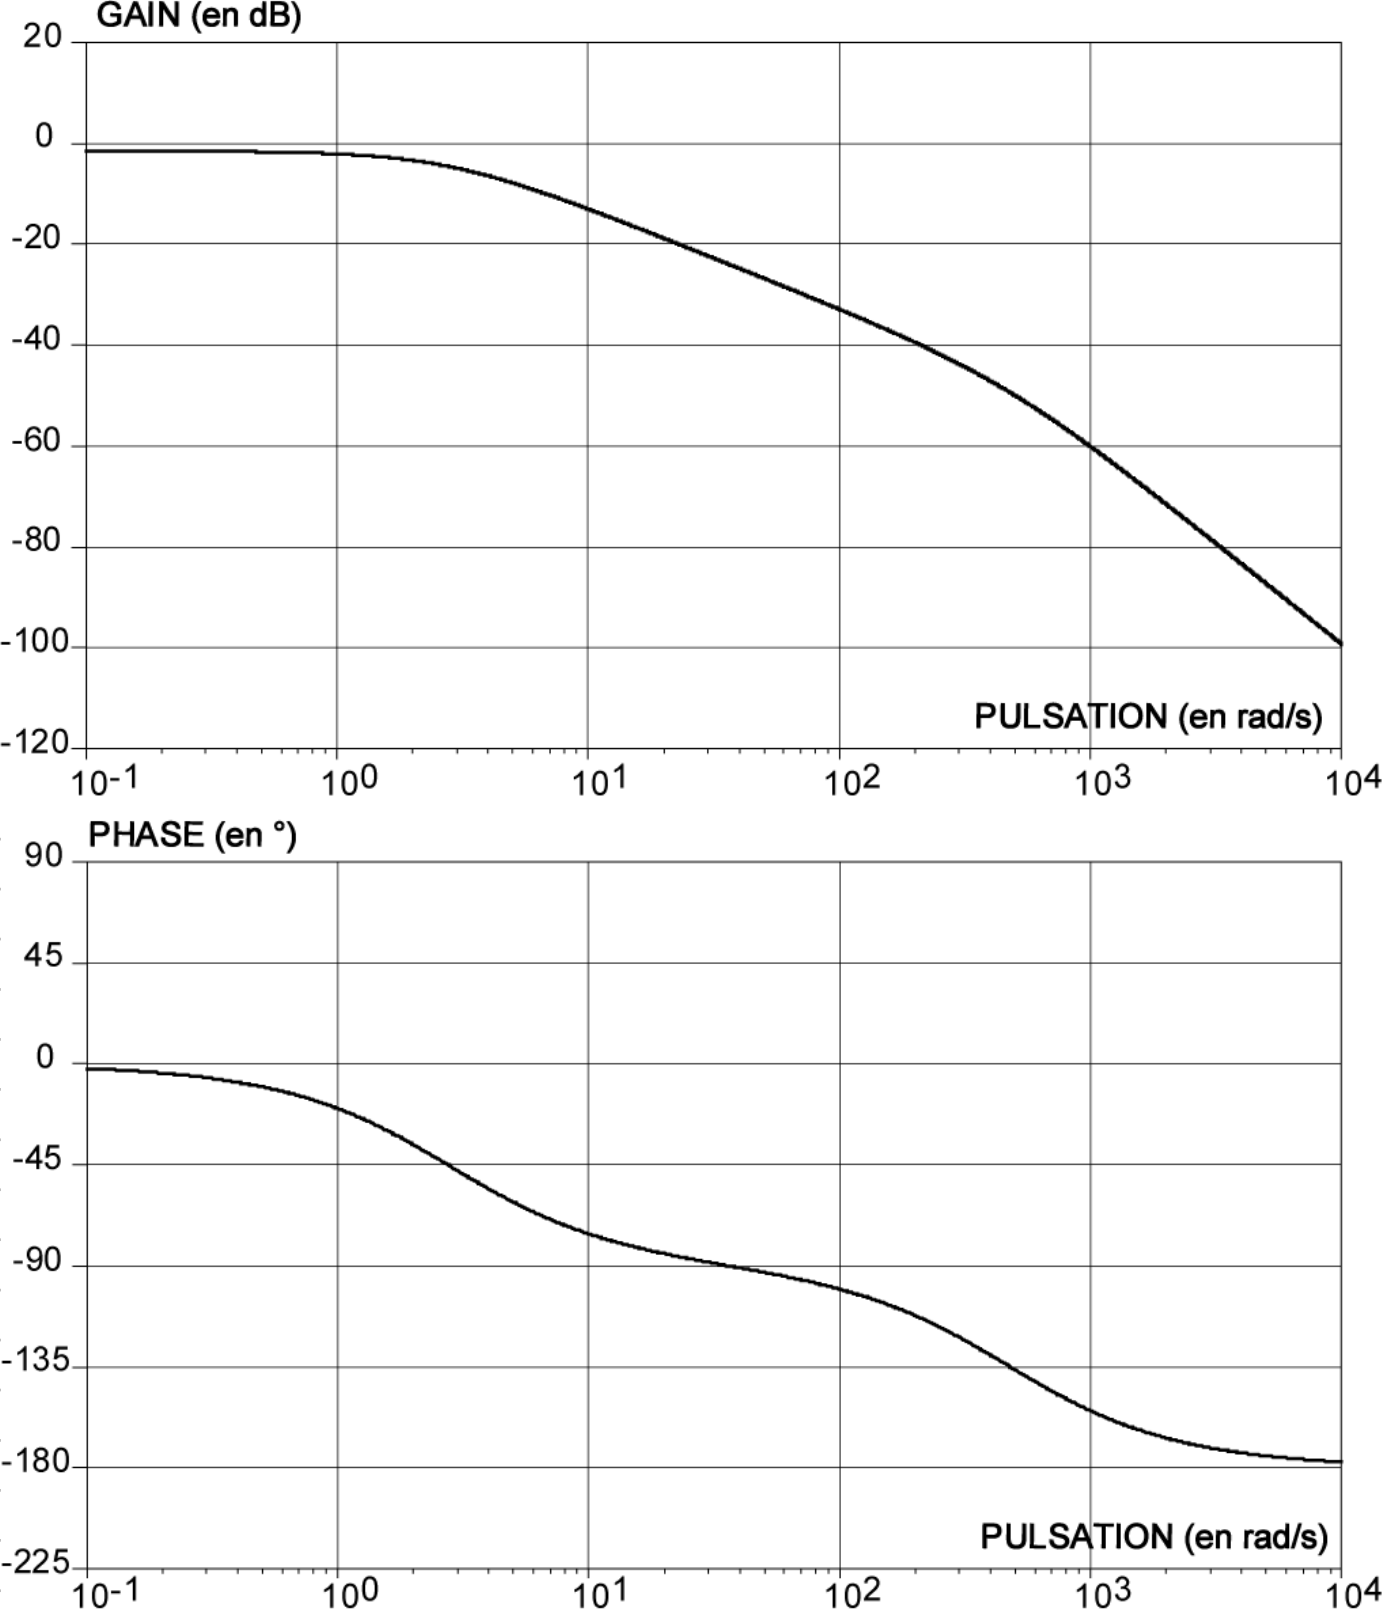
\includegraphics[width=.8\linewidth]{rep_q18}
\caption{Diagrame Bode de la boucle ouverte \label{rep_q_18}}
\end{figure}

\fi


\question{Etudier l’aptitude du système sans correction à respecter les critères de précision. Vous déterminerez notamment les expressions littérales de l’erreur statique en poursuite pour une consigne de vitesse de la plate-forme $V_c (t)$ en échelon d’amplitude $V_{\text{CO}}$ : $V_C (t)=V_{\text{CO}} u(t)$ (avec $u(t)$ l’échelon unitaire) et de l’influence en régulation d’une perturbation $C_{\text{equ}} (t)$ en échelon d’amplitude $C_0$, sur la vitesse réelle $V (t)$ de la plate-forme en régime permanent.}
\ifprof
\begin{corrige}
Le système est de classe 0. La précision en poursuite et en régulation ne peut donc pas être nulle.

Notons $\varepsilon(p)$ l'écart en sortie du premier comparateur. On a  
$\varepsilon(p) = V_c(p)-V(p)$

$=V_c(p)-\left(K_G\indice{K}{Capt}K_A H_u(p) \varepsilon(p)- \indice{C}{equ}(p)H_C(p) \right)\dfrac{1}{K_G}$ 

$\Leftrightarrow \varepsilon(p)\left( 1+ \indice{K}{Capt}K_A H_u(p)\right)=V_c(p)+  \dfrac{H_C(p)}{K_G}\indice{C}{equ}(p)$

$\Leftrightarrow \varepsilon(p)=\dfrac{1}{1+ \indice{K}{Capt}K_A H_u(p)}V_c(p)+ \dfrac{H_C(p)}{K_G+ K_G\indice{K}{Capt}K_A H_u(p)}\indice{C}{equ}(p)$.

Par ailleurs, $V_C (p)=\dfrac{V_{\text{CO}}}{p}$ et $C_{\text{equ}} (p) = \dfrac{C_0}{p}$.

On a donc $\varepsilon_S = \lim\limits_{p\to 0} p \varepsilon(p)$
$=\dfrac{1}{1+ \indice{K}{Capt}K_A K_U}V_{\text{CO}}+ \dfrac{K_C}{K_G+ K_G\indice{K}{Capt}K_A K_U}C_0$.
On a donc $\dfrac{V_{\text{CO}}}{1+ \indice{K}{Capt}K_A K_U}$ erreur en poursuite et 
$\dfrac{K_C C_0}{K_G+ K_G\indice{K}{Capt}K_A K_U}$ erreur en régulation.
\end{corrige}
\else
\fi


\subsubsection{Etude des performances avec un correcteur de fonction de transfert : $C(p)=\dfrac{K_I}{p}$}

\question{\label{q_20}Indiquer quelle est la nature de la correction effectuée par ce correcteur (ou désignation du correcteur) ? Indiquer pour quelle(s) raison(s) principale(s) ce correcteur a été choisi. Valider ce choix vis à vis du cahier des charges. Sans calcul, donner l’influence de ce correcteur sur les autres performances attendues.}
\ifprof
\begin{corrige}
Il s'agit d'un correcteur proportionnel intégral pur. 

Il annule l'écart statique. Il ajoute 90\degres de déphasage ce qui peut déstabiliser le système.
\end{corrige}
\else
\fi


Reprenons le diagramme de Bode de la Fonction de Transfert en Boucle Ouverte $\text{FTBO( p)}$ non corrigée (Bode non corrigé figure \ref{rep_q_18}).

\question{\label{q_21}Compléter le document-réponse (Bode non corrigé page 12) en traçant les diagrammes de Bode du correcteur avec $K_I =\SI{1}{s^{-1}}$ . Déterminer alors la valeur de $K_I$ maximale notée $K_{\text{I max}}$ permettant de respecter les marges de stabilité énoncées dans le cahier des charges.}
\ifprof
\begin{corrige}

\end{corrige}
\else
\fi


Afin d’évaluer analytiquement le temps de réponse à 5\%, Il est proposé d’adopter une modélisation simplifiée du
comportement du moteur en conservant uniquement le mode associé au pôle «~dominant~». On donne $T_{\SI{5}{\%} \text{mini}}\cdot \omega_0 = 3$ avec $\omega_0$ la pulsation propre non amortie d’un système fondamental du second ordre.

\question{\label{q_22}En analysant les valeurs numériques des pôles de la fonction de transfert du moteur en poursuite $H_U ( p)$, préciser quel est le pôle dominant et proposer alors un modèle simplifié de la fonction de transfert $H_U ( p)$. Déterminer alors la valeur numérique de $K_I$ notée $K_{I\SI{5}{\%}}$ minimisant le temps de réponse à \SI{5}{\%} pour une entrée échelon en poursuite. Calculer alors la valeur approchée du temps de réponse à \SI{5}{\%} minimale $T_{\SI{5}{\%} \text{mini}}$ et comparer la au cahier des charges.}
\ifprof
\begin{corrige}
\end{corrige}
\else
\fi



\subsubsection{Etude des performances avec un correcteur proportionnel intégral : $C(p)={K_P}\left(1+\dfrac{1}{T_I p}\right)$}

Le correcteur est remplacé par un correcteur proportionnel intégral. Des réponses temporelles du système corrigé sont tracées sur le document-réponse (question \ref{q_23}) avec :
\begin{itemize}
\item une consigne de vitesse unitaire de la plate-forme $V_c (t)= u(t)$ (avec $u(t)$ l’échelon unitaire) ;
\item une perturbation sous la forme d’un échelon unitaire retardé de 5 secondes $C_{\text{equ}} (t) = u(t - 5)$;
\item un gain du correcteur $K_P = 1$;
\item différentes valeurs de $T_I$.
\end{itemize}

\question{\label{q_23}Parmi les différentes valeurs de $T_I$, choisir celle qui assure le temps de réponse à 5\% le plus faible. Vous ferez apparaître ce temps de réponse sur la figure (question \ref{q_23}).}
\ifprof
\begin{corrige}
\end{corrige}
\else
\fi


La valeur de $T_I$ déterminée à la question précédente est retenue pour le réglage du correcteur proportionnel intégral. Il s’agit alors de choisir le gain du correcteur $K_P$ à partir des simulations proposées sur le document-réponse (question \ref{q_24}).

\question{\label{q_24}Parmi les différentes valeurs de $K_P$, choisir la valeur qui assure un temps de réponse à 5\% au plus près de la valeur fournie dans le cahier des charges.}
\ifprof
\begin{corrige}
\end{corrige}
\else
\fi


Avec le couple de valeurs ($T_I$ et $K_P$) obtenu, la réponse fréquentielle du système en boucle ouverte a été tracée sur le document réponse (question \ref{q_25}).

\question{\label{q_25} Conclure quant à la capacité de ce correcteur à respecter tous les critères du cahier des charges.}
\ifprof
\begin{corrige}
\end{corrige}
\else
\fi


%\section{Fonction technique FT33 : guider les podes en roulis}
\section{Exigence technique 1.3.3 : guider les podes en roulis}

L’objet de cette partie est d’étudier les solutions constructives assurant le guidage des podes en roulis. Ce guidage est réalisé par deux liaisons identiques, une pour le pode avant \textbf{3} et une pour le pode arrière \textbf{2}. Dans la suite, une seule des deux liaisons sera détaillée.

\subsection{Description de la première solution constructive (annexe 10)}

Les podes sont constitués d’un caisson creux dans lequel l’ensemble des éléments techniques prend place. Les caissons sont réalisés par assemblage et collage de plaques de composites de type « sandwich ». L’utilisation de ce
type de matériau garantit une bonne résistance aux efforts tout en maîtrisant la masse.
Pour des raisons d’encombrement (place à l’intérieur des podes), la liaison en roulis s’effectue uniquement sur l’épaisseur de la plaque en relation avec le bras d’articulation. Un insert métallique a été incorporé dans la plaque au niveau de la liaison avec le bras. Cette liaison réalisée par contact bilatéral direct peut être modélisée par l’association de deux liaisons en parallèle.
\begin{itemize}
\item D’une part, une liaison appui plan réalisée par contact bilatéral entre l’insert lié au pode et deux rondelles liées
au bras d’articulation ;
\item D’autre part, par une liaison sphère cylindre (linéaire annulaire) modélisant le centrage court entre l’insert lié
au pode et le palier de roulis lié au bras d’articulation.
\end{itemize}

\question{\label{q_26} Proposer un schéma cinématique représentant l’association des deux liaisons en parallèle. L’orientation des liaisons sera déterminée à partir de l’analyse technologique de la liaison. Montrer que la modélisation adoptée conduit alors à une liaison équivalente pivot isostatique.}
\ifprof
\begin{corrige}
\end{corrige}
\else
\fi



\subsection{Amélioration de la solution constructive (annexe 11)}

Lors des premiers essais, des détériorations localisées au niveau de l’insert métallique des plaques composites ont pu être observées, notamment en présence de moments importants dans la liaison autour de l’axe vertical. Afin de
renforcer la liaison, Il a été décidé de rajouter sur chaque pode avant / arrière deux pistes circulaires métalliques et sur chaque bras deux plots venant glisser respectivement sur chacune des pistes et récupérer une partie des efforts.
Dans un premier temps, chaque plot est considéré solidaire du bras d’articulation (liaison complète) et chaque contact entre un plot et une piste circulaire est modélisé par une liaison appui plan.

\question{\label{q_27} Déterminer le degré d’hyperstatisme de cette nouvelle solution. Proposer alors une solution modifiée sous la forme d’un schéma d’architecture (ou cinématique) permettant de réaliser les réglages géométriques nécessaires afin d’assurer un contact surfacique optimal entre chaque plot et la piste circulaire.}
\ifprof
\begin{corrige}
\end{corrige}
\else
\fi

	
\includepdf[pages=-]{Annexes.pdf}